\chapter{HASIL DAN PEMBAHASAN}
\label{chap:chap4_eval}
\vspace{1ex}

\section*{}
Inti dari BAB \ref{chap:chap4_eval} pada penelitian ini adalah pengujian dengan berbagai parameter atribut \textit{gameplay} yang dihasilkan untuk pemain dan musuh. Jika pada BAB \ref{chap:chap3_metodologi} dalam proses analisan desain permainan RPG, permainan RPG digolongkan berdasarkan pertarungan menjadi \textit{real-time} dan \textit{turn-based}.
\vspace{1ex}

Kemudian jika melihat jumlah karakter yang dimainkan oleh pemain maka permainan RPG dapat digolongkan menjadi \textit{single-character} dan \textit{multi-character}. Hal ini diperlukan dalam pengujian pembuatan atribut \textit{gameplay} yang dihasilkan, genre dari RPG yang termasuk \textit{single-character} adalah WRPG, ARPG, SRPG dan MMORPG, sedangkan yang termasuk \textit{multi-character} adalah TRPG dan JRPG. Sedangkan untuk karakter musuh dianggap sama. Dalam beberapa permainan bergenre RPG, pemain dan musuh tidak menggunakan sistem elemen sebagai kelemahan. Biasanya pada permainan RPG dengan genre ARPG, SRPG dan sebagian WRPG, sedangkan untuk TRPG dan JRPG hampir sebagian besar memakai sistem elemen sebagai kelemahan dalam sistem pertarungan.
\vspace{1ex}

\section{Hasil Atribut Gameplay Pemain (Single-Character)}
\label{sec:sec4_eval_single-character_player}
\vspace{1ex}

Pada bagian ini setiap langkah yang akan diuji sudah dijelaskan pada Sub-bab \ref{sec:sec3_player_stats}, dimana pada bagian ini membahas tentang pembuatan atribut \textit{gameplay} pemain untuk permaian bergenre RPG. Melalui berbagai proses seperti yang dijelaskan pada Sub-bab \ref{sec:sec3_player_stats}, maka pada beberapa Sub-bab dibawah ini adalah langkah-langkah dalam proses pengujiannya. Maksud dari \textit{single-character} disini adalah pemain hanya menjalankan satu buah karakter saja selama permainan, contoh dari RPG jenis ini biasanya ada pada WRPG, SRPG, ARPG, dan MMORPG.
\vspace{1ex}

\subsection{Hasil Distibusi Level, HP, dan MP Pemain}
\label{sec:sub_sec4_eval_dist_hp_mp_level_single-character}
\vspace{1ex}

Seperti yang sudah dijelaskan pada Sub-bab \ref{sec:sub_sec3_player_level_hp_mp}, yang membahas tentang pembuatan level, HP dan MP pemain untuk permaian dengan genre RPG. Berikut adalah hasil dari prosess pembuatan Level, HP, dan MP yang diperoleh dari perhitungan pada persamaan \ref{eq:hp_player} dan \ref{eq:mp_player} dengan data masukan pada Tabel \ref{tb:player_input_variable} yang kemudian menghasilkan data seperti yang ditunjukkan pada Tabel \ref{tb:player_hp_mp}.

\begin{longtable}{|l|l|l|}
	\caption{Hasil Perhitungan HP dan MP}
	\vspace{1ex}
	\label{tb:player_hp_mp}\\
	\hline
	\rowcolor[HTML]{C0C0C0} 
	\textbf{Levels} & \textbf{HP} & \textbf{MP} \\ \hline
	1 & 159 & 89 \\ \hline
	2 & 163 & 93 \\ \hline
	3 & 167 & 97 \\ \hline
	4 & 171 & 101 \\ \hline
	5 & 175 & 105 \\ \hline
	6 & 179 & 109 \\ \hline
	7 & 183 & 113 \\ \hline
	... & ... & ... \\ \hline
	\textbf{100} & \textbf{555} & \textbf{485} \\ \hline
\end{longtable}
\vspace{1ex}

Hasil perhitungan tersebut terlihat membentuk pola linier, yang mana nilai HP dan MP terus naik secara konstan ke atas sesuai dengan kenaikan levelnya seperti yang direpresentasikan pada Gambar \ref{fig:hp_player} dan Gambar \ref{fig:mp_player}. Jika melihat Gambar \ref{fig:hp_player} dengan jumlah HP dari pemain yang terus naik mengikuti pola yang dihasilkan pada Tabel \ref{tb:player_hp_mp}, yang mana nilai tersebut diperoleh dari inisiasi variabel pada Tabel \ref{tb:player_input_variable} yaitu \textit{Max Level}, \textit{Start HP} dan \textit{Next HP}. Variabel-variabel tersebut dihitung dengan menggunakan persamaan \ref{eq:hp_player} agar membentuk pola kenaikan HP setiap levelnya seperti yang ditunjukan pada Gambar \ref{fig:hp_player}. Sama seperti pada Gambar \ref{fig:hp_player}, pada Gambar \ref{fig:mp_player} dengan jumlah MP dari pemain yang terus naik mengikuti pola yang dihasilkan pada Tabel \ref{tb:player_hp_mp}, yang mana nilai tersebut diperoleh dari inisiasi variabel pada Tabel \ref{tb:player_input_variable} yaitu \textit{Max Level}, \textit{Start MP} dan \textit{Next MP}. Kemudian variabel-variabel tersebut dihitung dengan menggunakan persamaan \ref{eq:mp_player} agar membentuk pola kenaikan MP setiap levelnya seperti yang ditunjukan pada Gambar \ref{fig:mp_player}. 
\vspace{1ex}

\begin{figure} [!h] \centering
	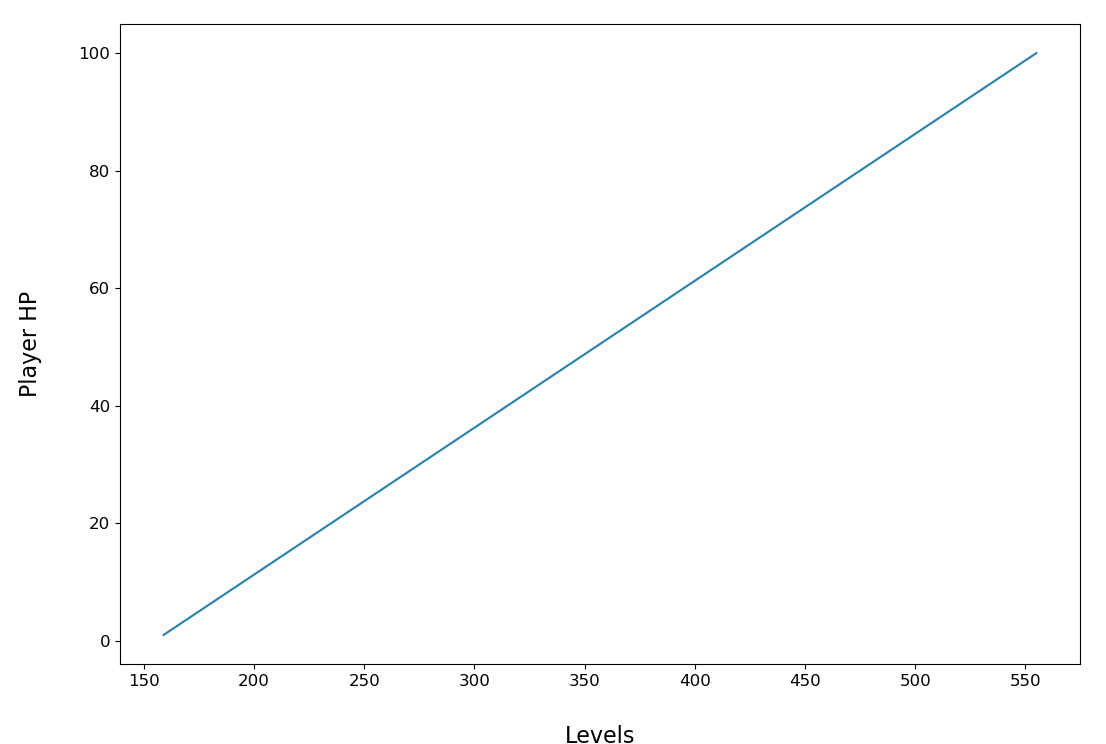
\includegraphics[scale=0.44]{img/PlayerHpDistrib.png}
	\caption{Kenaikan HP setiap levelnya.}
	\label{fig:hp_player}
\end{figure}

\begin{figure} [!h] \centering
	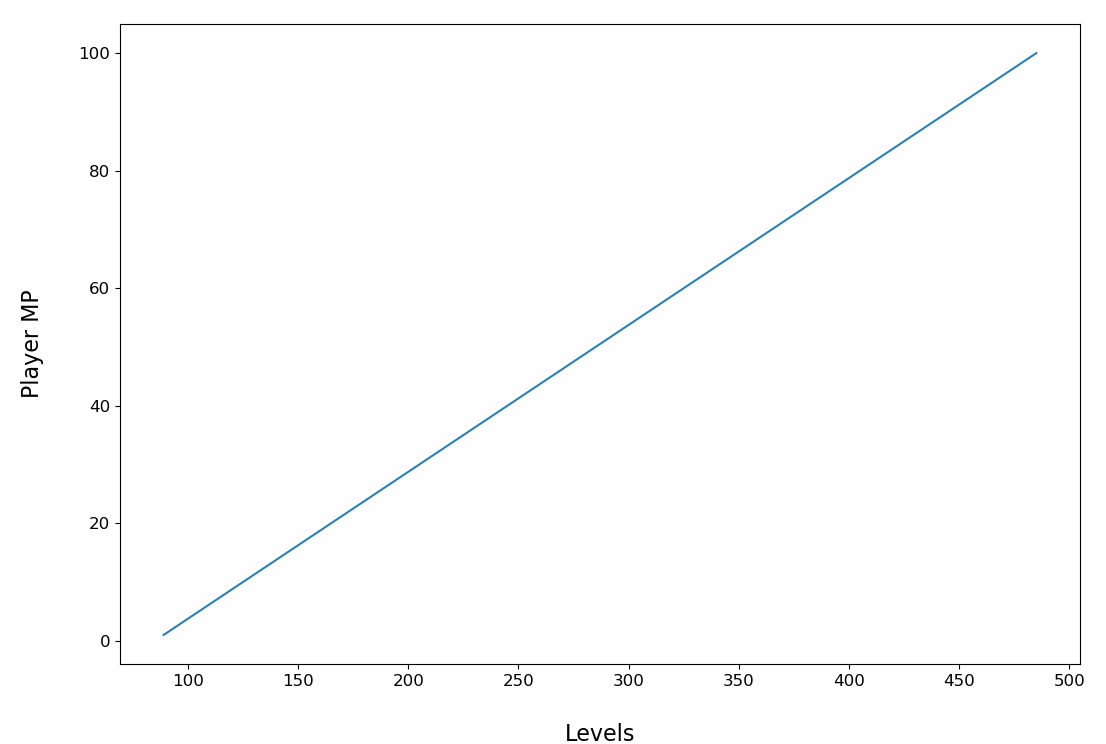
\includegraphics[scale=0.44]{img/PlayerMpDistrib.png}
	\caption{Kenaikan MP setiap levelnya.}
	\label{fig:mp_player}
\end{figure}

Pada setiap proses pengujian dalam Sub-bab ini, yang dihasilkan pada Tabel \ref{tb:player_hp_mp} menyajikan sebagian data saja. Hasil selengkapnya dapat dilihat pada Tabel \ref{tb:player_hp_mp_all} dalam \nameref{chap:chap6_attachment} yang kemudian keseluruhan hasil tersebut divisualisasikan pada Gambar \ref{fig:hp_player}.
\vspace{1ex}

\subsection{Hasil Distibusi Elemen dan Kelemahan Pemain}
\label{sec:sub_sec4_eval_dist_element_single-character}
\vspace{1ex}

Pada bagian ini hanya akan mengulas tentang distribusi elemen dan kelemahan pemain pada Sub-Bab \ref{sec:sub_sec3_list_element_player}, yang sejatinya didefinisikan secara manual pada program yang dibuat dan dijelaskan pada Sub-Bab \ref{sec:sec3_player_stats}. Di mana elemen pada permainan RPG bersifat opsional, tidak dibatasi apakah permainan RPG tersebut tergolong ke dalam \textit{turn-base} atau \textit{real-time}, tergolong \textit{singe-character} atau \textit{multi-character}. Hal tersebut murni bergantung pada pengembang dan desainer permainan. Maka dari itu melalui program yang dibuat pada Sub-Bab \ref{sec:sec3_player_stats} hal ini diwujudkan dalam bentuk opsi yang dapat digunakan atau ditinggalkan, sesuai kebutuhan pengembang atau desainer permainan. Bila opsi distribusi elemen digunakan maka hasilnya akan tampak seperti pada Tabel \ref{tb:player_element}, dengan asumsi tidak adanya perubahan elemen dari karakter pemain dalam permainan.
\vspace{-1ex}

\begin{longtable}{|l|l|l|l|l|l|}
	\caption{Distribusi elemen pada karakter pemain}
	\vspace{1ex}
	\label{tb:player_element}\\
	\hline
	\rowcolor[HTML]{C0C0C0} 
	\multicolumn{1}{|c|}{\cellcolor[HTML]{C0C0C0}\textbf{Levels}} & \multicolumn{1}{c|}{\cellcolor[HTML]{C0C0C0}\textbf{Water}} & \multicolumn{1}{c|}{\cellcolor[HTML]{C0C0C0}\textbf{Wind}} & \multicolumn{1}{c|}{\cellcolor[HTML]{C0C0C0}\textbf{Earth}} & \multicolumn{1}{c|}{\cellcolor[HTML]{C0C0C0}\textbf{Fire}} \\ \hline
	1 & 2 & 0 & 0 & 1 \\ \hline
	2 & 2 & 0 & 0 & 1 \\ \hline
	3 & 2 & 0 & 0 & 1 \\ \hline
	4 & 2 & 0 & 0 & 1 \\ \hline
	5 & 2 & 0 & 0 & 1 \\ \hline
	6 & 2 & 0 & 0 & 1 \\ \hline
	7 & 2 & 0 & 0 & 1 \\ \hline
	... & ... & ... & ... & ... \\ \hline
	\textbf{100} & \textbf{2} & \textbf{0} & \textbf{0} & \textbf{1} \\ \hline
\end{longtable}

Pada setiap proses pengujian dalam Sub-bab ini, yang dihasilkan pada Tabel \ref{tb:player_element} menyajikan sebagian data saja. Hasil selengkapnya dapat dilihat pada Tabel \ref{tb:player_all_stats_1} sampai dengan Tabel \ref{tb:player_all_stats_4} dalam \nameref{chap:chap6_attachment}. Hal seperti penggunaan elemen pada pemain seperti pembahasan pada Sub-bab ini an sebelumnya, biasanya dijumpai pada permain RPG dengan Sub-genre JRPG, TRPG, WRPG dan MMORPG. Namun itu juga tidak semua permainan RPG dengan genre tersebut menggunakannya, hanya yang sering dijumpai saja.
\vspace{1ex}

\subsection{Hasil Distibusi Atribut Gameplay Pemain}
\label{sec:sub_sec4_eval_single-character_stats}
\vspace{1ex}

Pada bagian ini setiap langkah yang akan diuji sudah dijelaskan pada Sub-bab \ref{sec:sub_sec3_stat_pemain}, dimana pada bagian ini membahas tentang pembuatan atribut \textit{gameplay} pemain untuk permaian RPG. Melalui berbagai proses seperti yang dijelaskan pada Sub-bab \ref{sec:sub_sec3_stat_pemain}, melalui data masukan pada Tabel \ref{tb:player_input_variable} kemudian persamaan \ref{eq:KNN_bayes_player_stats} dan beberapa persamaan lain yang disebutkan pada Sub-bab \ref{sec:sub_sec3_stat_pemain} dihasilkan data seperti yang ditunjukan pada Tabel \ref{tb:player_battle_stats}.
\vspace{-1ex}

\begin{longtable}{|l|l|l|l|l|l|}
	\caption{Distribusi atribut \textit{gameplay} pada karakter pemain}
	\vspace{1ex}
	\label{tb:player_battle_stats}\\
	\hline
	\rowcolor[HTML]{C0C0C0} 
	\textbf{Levels} & \textbf{Strength} & \textbf{Magic} & \textbf{Endurance} & \textbf{Speed} & \textbf{Luck} \\ \hline
	1 & 1 & 2 & 0 & 0 & 1 \\ \hline
	2 & 0 & 2 & 0 & 2 & 0 \\ \hline
	3 & 1 & 0 & 0 & 0 & 0 \\ \hline
	4 & 1 & 1 & 0 & 0 & 0 \\ \hline
	5 & 1 & 1 & 0 & 0 & 0 \\ \hline
	6 & 1 & 1 & 0 & 2 & 1 \\ \hline
	7 & 0 & 0 & 0 & 0 & 1 \\ \hline
	... & ... & ... & ... & ... & ... \\ \hline
	\textbf{100} & \textbf{74} & \textbf{38} & \textbf{63} & \textbf{65} & \textbf{60} \\ \hline
\end{longtable}
\vspace{1ex}

Pada Tabel \ref{tb:player_battle_stats} adalah data distribusi atribut \textit{gameplay} dari pemain yang dihasilakn melalui penambahan nilai pada atribut \textit{gameplay} secara acak pada setiap atribut \textit{gameplay}. Seperti yang dijelaskan pada persaamaan \ref{eq:nbayes_class}, \ref{eq:KNN_distance_stats}, dan persamaan \ref{eq:KNN_bayes_player_stats} saat nilai atribut \textit{gameplay} ditambahkan secara acak dari 1 sampai dengan 2 pada level yang berjarak antara 1 sampai dengan 100. Selanjutnya representasi dari hasil penambahan atribut \textit{gameplay} tersebut yang ditunjukan melalui Gambar \ref{fig:stats_player} yang mana nilai dari setiap atribut \textit{gameplay} terus naik sesuai dengan level pemain yang juga terus naik. 
\vspace{1ex}

\begin{figure} [!h] \centering
	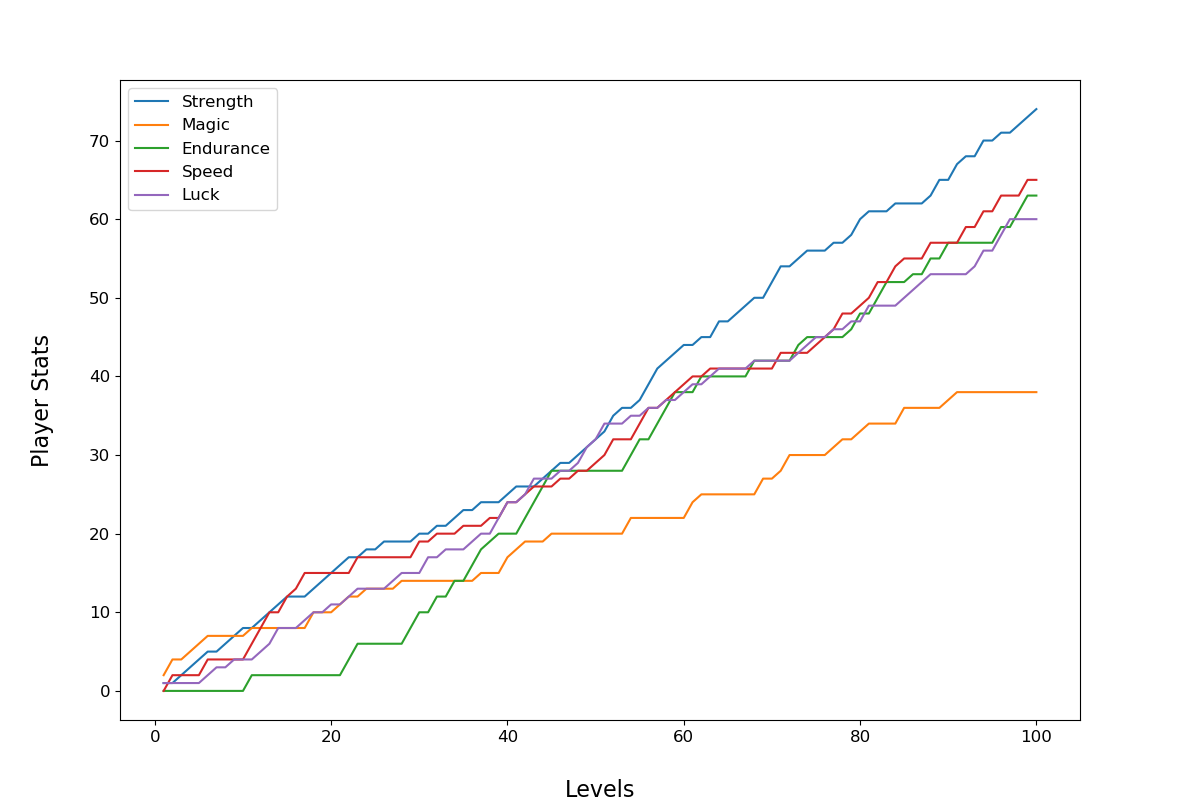
\includegraphics[scale=0.45]{img/PlayerStatsDistrib.png}
	\caption{Kenaikan atribut \textit{gameplay} pemain setiap levelnya.}
	\label{fig:stats_player}
\end{figure}

Pada setiap proses pengujian dalam Sub-bab ini, yang dihasilkan pada Tabel \ref{tb:player_battle_stats} menyajikan sebagian data saja. Hasil selengkapnya dapat dilihat pada Tabel \ref{tb:player_all_stats_1} sampai dengan Tabel \ref{tb:player_all_stats_4} dalam \nameref{chap:chap6_attachment} yang kemudian keseluruhan hasil tersebut divisualisasikan pada Gambar \ref{fig:stats_player}.
\vspace{1ex}

\section{Hasil Atribut Gameplay Pemain (Multi-Character)}
\label{sec:sec4_eval_multi-character_player}
\vspace{1ex}

Pada bagian ini setiap langkah yang akan diuji sudah dijelaskan pada Sub-bab \ref{sec:sec3_player_stats}, dimana pada bagian ini membahas tentang pembuatan atribut \textit{gameplay} pemain untuk permaian dengan genre RPG. Melalui berbagai proses seperti yang dijelaskan pada Sub-bab \ref{sec:sec3_player_stats}, maka pada beberapa Sub-bab dibawah ini adalah langkah-langkah dalam proses pengujiannya. Maksud dari Multi-Character disini adalah pemain dapat menjalankan beberapa karakter sekaligus, menjalankan dengan mode \textit{turn-based} atau \textit{switch} antar karakter seperti yang dijelaskan pada Sub-Bab \ref{sec:sub_sec2_jrpg}. Maka dari itu dibuatlah Tabel masukan baru pada Tabel \ref{tb:player_input_variable_eval_1} dan \ref{tb:player_input_variable_eval_2} yang mirip seperti Tabel \ref{tb:player_input_variable}. Hal ini bertujuan membandingkan perbedaan atribut \textit{gameplay} yang dihasilkan pada tiga karakter pemain.
\vspace{-2ex}

\begin{longtable}{|l|l|}
	\caption{Data masukan untuk pembuatan atribut \textit{gameplay} karakter pertama.}
	\vspace{1ex}
	\label{tb:player_input_variable_eval_1}\\
	\hline
	\rowcolor[HTML]{9B9B9B}
	\multicolumn{1}{|c|}{\cellcolor[HTML]{9B9B9B}\textbf{Variabel}} & \multicolumn{1}{c|}{\cellcolor[HTML]{9B9B9B}\textbf{Input}} \\ \hline
	\textit{Start} Level & 1 \\ \hline
	\textit{Max} Level & 100 \\ \hline
	\textit{Start} HP & 224 \\ \hline
	\textit{Next} HP & 228 \\ \hline
	\textit{Start} MP & 100 \\ \hline
	\textit{Next} MP & 102 \\ \hline
	\textit{List Element} & {[} `Phys', `Water', `Wind', `Earth', `Fire' {]} \\ \hline
	\textit{List Weaknesess} & {[} 0, 0, 2, 1, 0 {]} \\ \hline
	\textit{List Attributes Name} & {[} `Strength', `Magic', `Endurance', `Speed', `Luck' {]} \\ \hline
	\textit{Max Attributes Value} & {[} 88, 32, 81, 43, 56 {]} \\ \hline
	\textit{Attributes to Assign} & {[} 2, 1 {]} \\ \hline
\end{longtable}
\vspace{-2ex}

\begin{longtable}{|l|l|}
	\caption{Data masukan untuk pembuatan atribut \textit{gameplay} karakter kedua.}
	\vspace{1ex}
	\label{tb:player_input_variable_eval_2}\\
	\hline
	\rowcolor[HTML]{9B9B9B} 
	\multicolumn{1}{|c|}{\cellcolor[HTML]{9B9B9B}\textbf{Variabel}} & \multicolumn{1}{c|}{\cellcolor[HTML]{9B9B9B}\textbf{Input}} \\ \hline
	\textit{Start} Level & 1 \\ \hline
	\textit{Max} Level & 100 \\ \hline
	\textit{Start} HP & 223 \\ \hline
	\textit{Next} HP & 226 \\ \hline
	\textit{Start} MP & 154 \\ \hline
	\textit{Next} MP & 158 \\ \hline
	\textit{List Element} & {[} `Phys', `Water', `Wind', `Earth', `Fire' {]} \\ \hline
	\textit{List Weaknesess} & {[} 0, 1, 0, 0, 2 {]} \\ \hline
	\textit{List Attributes Name} & {[} `Strength', `Magic', `Endurance', `Speed', `Luck' {]} \\ \hline
	\textit{Max Attributes Value} & {[} 60, 68, 57, 58, 57 {]} \\ \hline
	\textit{Attributes to Assign} & {[} 2, 1 {]} \\ \hline
\end{longtable}
\vspace{1ex}

Kemudian dari Tabel \ref{tb:player_input_variable_eval_1} dan Tabel \ref{tb:player_input_variable_eval_2} dihasilkan dua atribut \textit{gameplay} yang berbeda untuk dua karakter dari pemain. Pada mulanya pemilihan atribut \textit{gameplay} pemain yang dinyatakan pada ke dua Table tersebut bukanlah tidak beralasan, bila melihat pada Tabel yang sebelumnya dipakai untuk pengujian \textit{single-character} pada Sub-bab \ref{sec:sec4_eval_single-character_player} dan penjabaran metodologi pembuatan atribut \textit{gameplay} karakter pemain pada Sub-bab \ref{sec:sec3_player_stats} tentu saja masih berkaitan. Ketiga atribut \textit{gameplay} tersebut membentuk sebuah \textit{party member} dalam permainan JRPG atau bahkan TRPG, hal ini sengaja dibuat dikarenakan hanya genre permainan RPG tersebut yang memungkinkan pemain menggunakan lebih dari satu karakter. Penjelasaan dan penggunaan dari ke empat atribut \textit{gameplay} tersebut akan diperjelas pada beberapa Sub-bab berikut ini.
\vspace{1ex}

\subsection{Hasil Distibusi Level, HP, dan MP Pemain}
\label{sec:sub_sec4_eval_dist_hp_mp_level_multi-character}
\vspace{1ex}

Seperti yang sudah dijelaskan pada Sub-bab \ref{sec:sub_sec3_player_level_hp_mp}, dimana pada bagian ini membahas tentang pembuatan level, HP dan MP pemain untuk permaian dengan genre RPG. Sama seperti pembahasan pada Sub-bab \ref{sec:sub_sec4_eval_dist_hp_mp_level_single-character}, hanya saja pada bagian ini, karakter pemain berjumlah lebih banyak dari pembahasan sebelumnya. Berikut adalah hasil dari prosess pembuatan Level, HP, dan MP yang diperoleh dari perhitungan pada persamaan \ref{eq:hp_player} dan \ref{eq:mp_player} dengan data masukan pada Tabel \ref{tb:player_input_variable_eval_1} dan Tabel \ref{tb:player_input_variable_eval_2} yang kemudian menghasilkan data seperti yang ditunjukkan pada Tabel \ref{tb:player_hp_mp_1} dan Tabel \ref{tb:player_hp_mp_2}.
\vspace{-1ex}

\begin{longtable}{|l|l|l|}
	\caption{Hasil Perhitungan HP dan MP karakter pertama}
	\vspace{1ex}
	\label{tb:player_hp_mp_1}\\
	\hline
	\rowcolor[HTML]{C0C0C0} 
	\textbf{Levels} & \textbf{HP} & \textbf{MP} \\ \hline
	1 & 224 & 100 \\ \hline
	2 & 228 & 102 \\ \hline
	3 & 232 & 104 \\ \hline
	4 & 236 & 106 \\ \hline
	5 & 240 & 108 \\ \hline
	6 & 244 & 110 \\ \hline
	7 & 248 & 112 \\ \hline
	... & ... & ... \\ \hline
	\textbf{100} & \textbf{620} & \textbf{298} \\ \hline
\end{longtable}
\vspace{1ex}

\begin{longtable}{|l|l|l|}
	\caption{Hasil Perhitungan HP dan MP karakter kedua}
	\vspace{1ex}
	\label{tb:player_hp_mp_2}\\
	\hline
	\rowcolor[HTML]{C0C0C0} 
	\textbf{Levels} & \textbf{HP} & \textbf{MP} \\ \hline
	1 & 223 & 154 \\ \hline
	2 & 226 & 158 \\ \hline
	3 & 229 & 162 \\ \hline
	4 & 232 & 166 \\ \hline
	5 & 235 & 170 \\ \hline
	6 & 238 & 174 \\ \hline
	7 & 241 & 178 \\ \hline
	... & ... & ... \\ \hline
	\textbf{100} & \textbf{520} & \textbf{550} \\ \hline
\end{longtable}
\vspace{1ex}

Hasil perhitungan tersebut terlihat membentuk pola linier, yang mana nilai HP terus naik secara konstan ke atas sesuai dengan kenaikan levelnya seperti yang direpresentasikan pada Gambar \ref{fig:hp_player_1}, dan Gambaer \ref{fig:hp_player_2}. Jika melihat Gambar \ref{fig:hp_player_1} dan Gambar \ref{fig:hp_player_2} dengan jumlah HP dari pemain yang terus naik mengikuti pola yang dihasilkan pada Tabel \ref{tb:player_hp_mp_1} dan Tabel \ref{tb:player_hp_mp_2}, yang mana nilai tersebut diperoleh dari inisiasi variabel pada Tabel \ref{tb:player_input_variable_eval_1} dan Tabel \ref{tb:player_input_variable_eval_2} yaitu \textit{Max Level}, \textit{Start} HP dan \textit{Next} HP. Variabel-variabel tersebut dihitung dengan menggunakan persamaan \ref{eq:hp_player} agar membentuk pola kenaikan HP setiap levelnya seperti yang ditunjukan pada Gambar \ref{fig:hp_player_1} dan Gambar \ref{fig:hp_player_2}. 
\vspace{1ex}

\begin{figure} [!h] \centering
	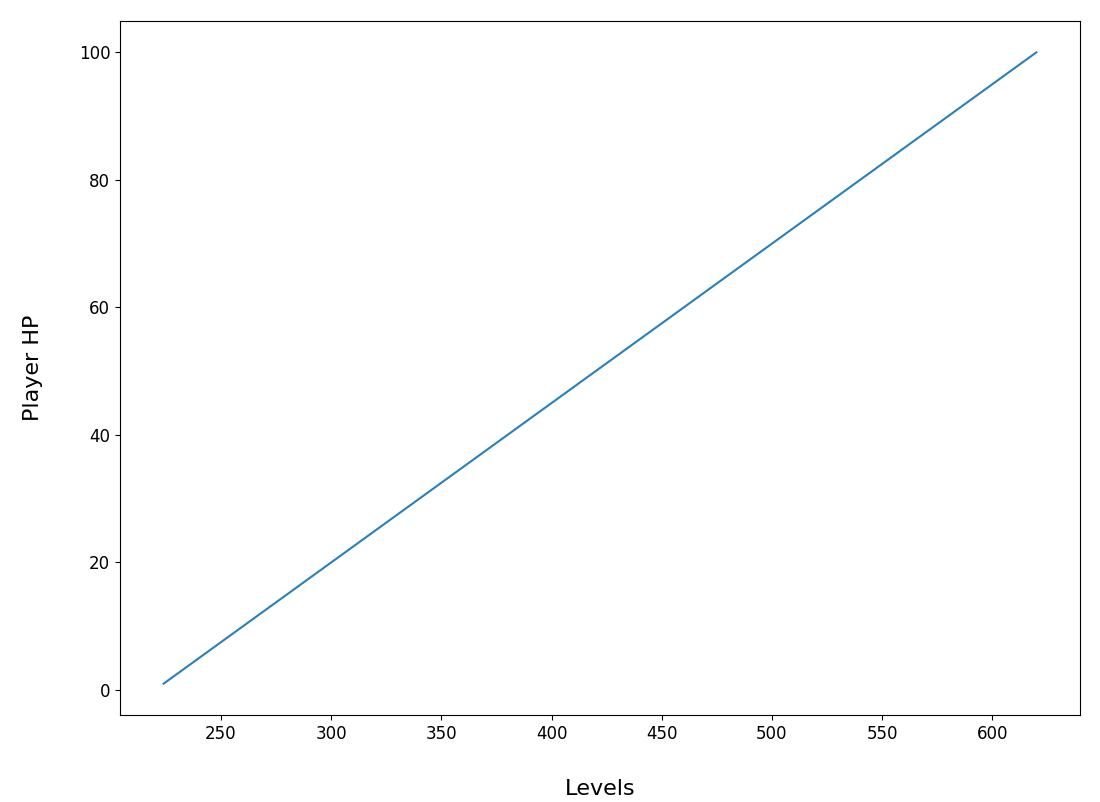
\includegraphics[scale=0.42]{img/PlayerHpDistrib1.png}
	\caption{Kenaikan HP setiap levelnya pada karakter pertama.}
	\label{fig:hp_player_1}
\end{figure}

\begin{figure} [!h] \centering
	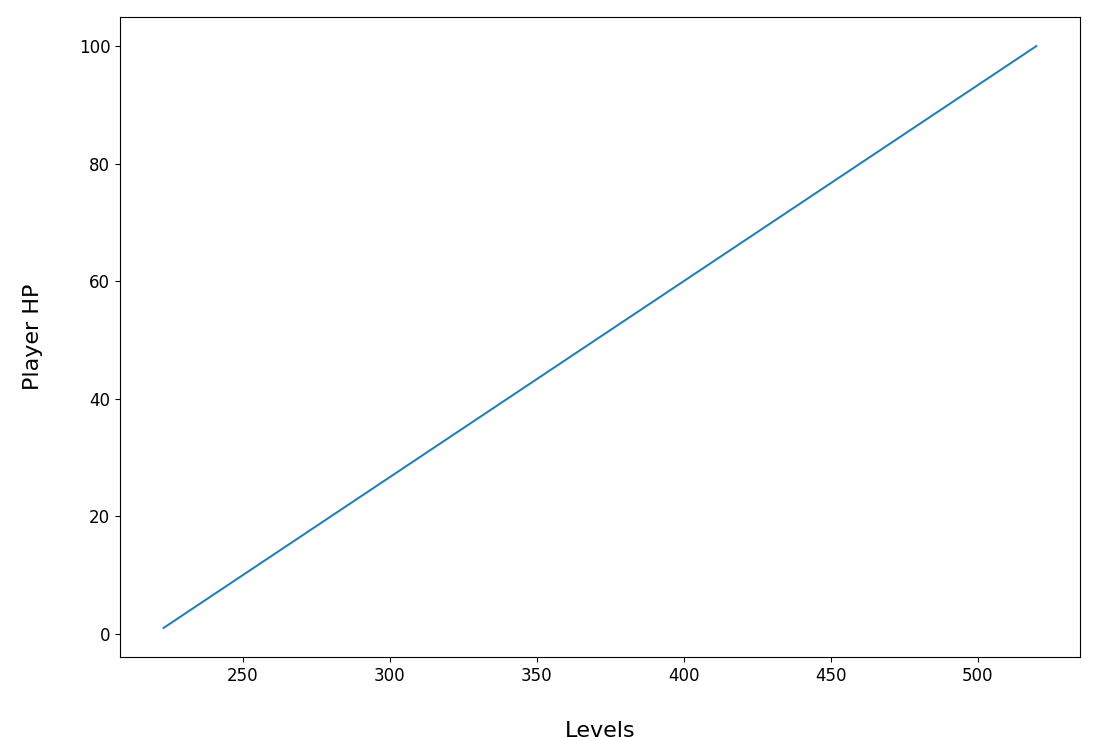
\includegraphics[scale=0.42]{img/PlayerHpDistrib2.png}
	\caption{Kenaikan HP setiap levelnya pada karakter kedua.}
	\vspace{1ex}
	\label{fig:hp_player_2}
\end{figure}

Sama seperti pada Gambar \ref{fig:mp_player_1} dan Gambar \ref{fig:mp_player_2} dengan jumlah MP dari pemain yang terus naik mengikuti pola yang dihasilkan pada Tabel \ref{tb:player_hp_mp_1} dan Tabel \ref{tb:player_hp_mp_2}, yang mana nilai tersebut diperoleh dari inisiasi variabel pada Tabel \ref{tb:player_input_variable} yaitu \textit{Max Level}, \textit{Start} MP dan \textit{Next} MP. Kemudian variabel-variabel tersebut dihitung dengan menggunakan persamaan \ref{eq:mp_player} agar membentuk pola kenaikan MP setiap levelnya seperti yang ditunjukan pada Gambar \ref{fig:mp_player_1} dan Gambar \ref{fig:mp_player_2}. 
\vspace{1ex}

\begin{figure} [!h] \centering
	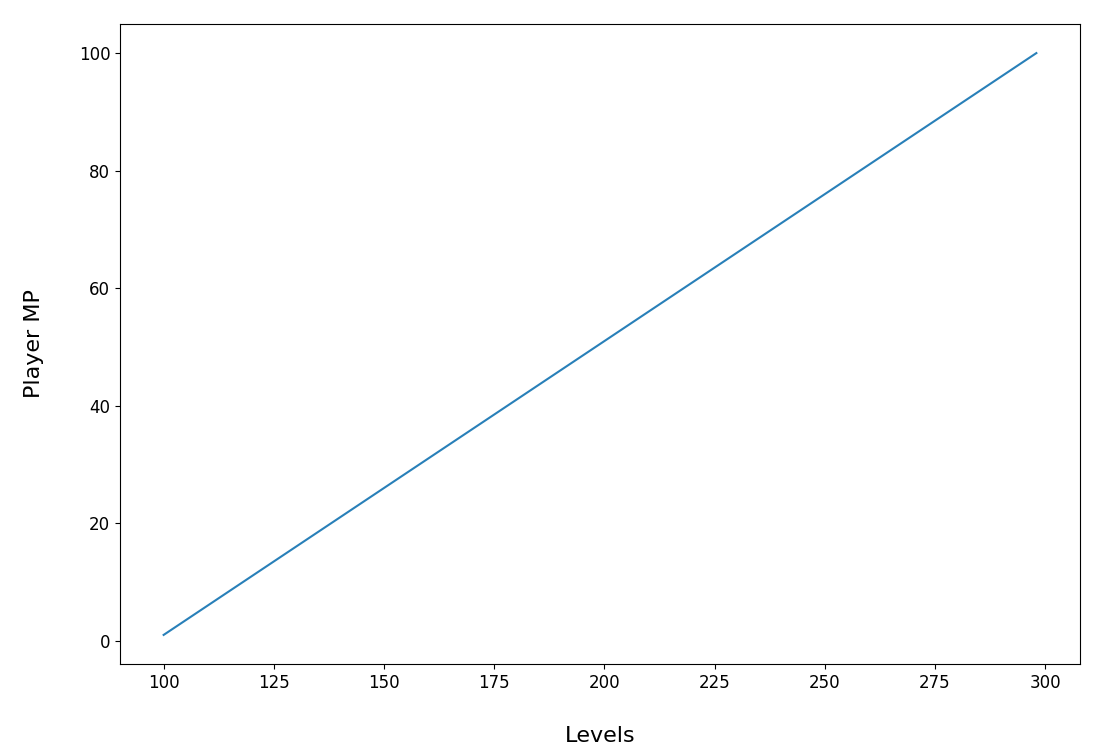
\includegraphics[scale=0.42]{img/PlayerMpDistrib1.png}
	\caption{Kenaikan MP setiap levelnya pada karakter pertama.}
	\label{fig:mp_player_1}
\end{figure}

\begin{figure} [!h] \centering
	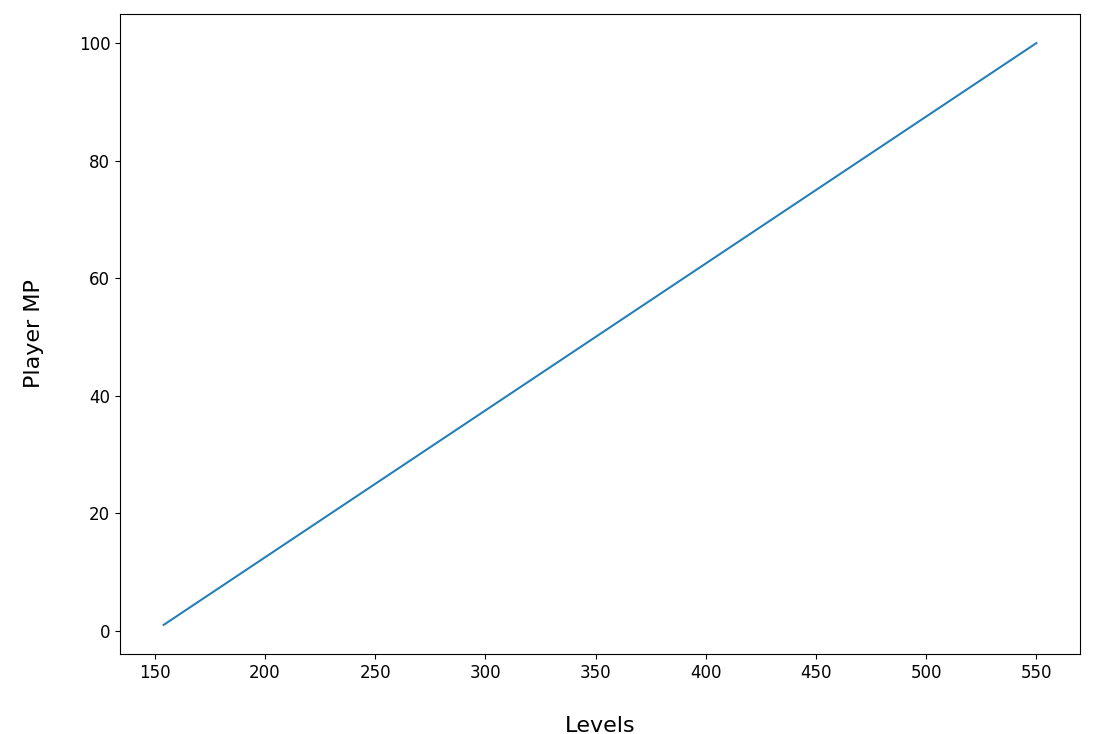
\includegraphics[scale=0.42]{img/PlayerMpDistrib2.png}
	\caption{Kenaikan MP setiap levelnya pada karakter kedua.}
	\label{fig:mp_player_2}
\end{figure}

Pada setiap proses pengujian dalam Sub-bab ini, yang dihasilkan pada Tabel \ref{tb:player_hp_mp_1} dan \ref{tb:player_hp_mp_2} menyajikan sebagian data saja. Hasil selengkapnya dapat dilihat pada Tabel \ref{tb:player_hp_mp_all_1} untuk karakter pertama dan pada \ref{tb:player_hp_mp_all_2} untuk karakter kedua yang terlampir dalam \nameref{chap:chap6_attachment}. Kemudian keseluruhan hasil tersebut divisualisasikan pada Gambar \ref{fig:hp_player_1}, dan Gambar \ref{fig:hp_player_2} untuk HP, Gambar \ref{fig:mp_player_1}, dan Gambar \ref{fig:mp_player_2} untuk MP.
\vspace{1ex}

\subsection{Hasil Distibusi Elemen dan Kelemahan Pemain}
\label{sec:sub_sec4_eval_dist_element_multi-character}
\vspace{1ex}

Sama seperti penjelasan pada Sub-bab \ref{sec:sub_sec4_eval_dist_element_single-character}, bila opsi distribusi elemen digunakan maka hasilnya akan tampak seperti pada Tabel \ref{tb:player_element_1} yang mengacu pada inputan dari Tabel \ref{tb:player_input_variable_eval_1} untuk karakter pemain pertama, sedangkan unt karakter pemain kedua hasilnya seperti pada Tabel \ref{tb:player_element_2} yang mengacu pada inputan dari Tabel \ref{tb:player_input_variable_eval_2}. Keduanya diasumsikan tidak adanya perubahan elemen dari karakter pemain dalam permainan.
\vspace{-1ex}

\begin{longtable}{|l|l|l|l|l|l|}
	\caption{Distribusi elemen pada karakter pemain pertama}
	\vspace{1ex}
	\label{tb:player_element_1}\\
	\hline
	\rowcolor[HTML]{C0C0C0} 
	\textbf{Phys} & \textbf{Water} & \textbf{Wind} & \textbf{Earth} & \textbf{Fire} \\ \hline
	0 & 0 & 2 & 1 & 0 \\ \hline
	0 & 0 & 2 & 1 & 0 \\ \hline
	0 & 0 & 2 & 1 & 0 \\ \hline
	0 & 0 & 2 & 1 & 0 \\ \hline
	0 & 0 & 2 & 1 & 0 \\ \hline
	0 & 0 & 2 & 1 & 0 \\ \hline
	... & ... & ... & ... & ... \\ \hline
	\textbf{0} & \textbf{0} & \textbf{2} & \textbf{1} & \textbf{0} \\ \hline
\end{longtable}
\vspace{-1ex}

\begin{longtable}{|l|l|l|l|l|l|}
	\caption{Distribusi elemen pada karakter pemain kedua}
	\vspace{1ex}
	\label{tb:player_element_2}\\
	\hline
	\rowcolor[HTML]{C0C0C0} 
	\textbf{Phys} & \textbf{Water} & \textbf{Wind} & \textbf{Earth} & \textbf{Fire} \\ \hline
	0 & 1 & 0 & 0 & 2 \\ \hline
	0 & 1 & 0 & 0 & 2 \\ \hline
	0 & 1 & 0 & 0 & 2 \\ \hline
	0 & 1 & 0 & 0 & 2 \\ \hline
	0 & 1 & 0 & 0 & 2 \\ \hline
	0 & 1 & 0 & 0 & 2 \\ \hline
	... & ... & ... & ... & ... \\ \hline
	\textbf{0} & \textbf{0} & \textbf{2} & \textbf{1} & \textbf{0} \\ \hline
\end{longtable}
\vspace{1ex}

Pada setiap proses pengujian dalam Sub-bab ini, yang dihasilkan pada Tabel \ref{tb:player_element_1} dan \ref{tb:player_element_2} menyajikan sebagian data saja. Hasil selengkapnya dapat dilihat pada Tabel \ref{tb:player_all_stats_1} sampai dengan Tabel \ref{tb:player_all_stats_4} dalam \nameref{chap:chap6_attachment}. Hal seperti penggunaan elemen pada pemain seperti pembahasan pada Sub-bab ini an sebelumnya, biasanya dijumpai pada permain RPG dengan Sub-genre JRPG, TRPG, WRPG dan MMORPG. Namun itu juga tidak semua permainan RPG dengan genre tersebut menggunakannya, hanya yang sering dijumpai saja.
\vspace{1ex}

\subsection{Hasil Distibusi Atribut Gameplay Pemain}
\label{sec:sub_sec4_eval_multi-character_stats}
\vspace{1ex}

Pada bagian ini setiap langkah yang akan diuji sudah dijelaskan pada Sub-bab \ref{sec:sub_sec3_stat_pemain}, dimana pada bagian ini membahas tentang pembuatan atribut \textit{gameplay} pemain untuk permaian RPG. Melalui berbagai proses seperti yang dijelaskan pada Sub-bab \ref{sec:sub_sec3_stat_pemain}, melalui data masukan pada Tabel \ref{tb:player_input_variable_eval_1} untuk karakter pertama dan Tabel \ref{tb:player_input_variable_eval_1} untuk karakter kedua, kemudian persamaan \ref{eq:KNN_bayes_player_stats} dan beberapa persamaan lain yang disebutkan pada Sub-bab \ref{sec:sub_sec3_stat_pemain} dihasilkan data seperti yang ditunjukan pada Tabel \ref{tb:player_battle_stats_1} dan Tabel \ref{tb:player_battle_stats_2}.
\vspace{-1ex}

\begin{longtable}{|l|l|l|l|l|l|}
	\caption{Distribusi atribut \textit{gameplay} pada karakter pertama pemain}
	\vspace{1ex}
	\label{tb:player_battle_stats_1}\\
	\hline
	\rowcolor[HTML]{C0C0C0} 
	\textbf{Levels} & \textbf{Strength} & \textbf{Magic} & \textbf{Endurance} & \textbf{Speed} & \textbf{Luck} \\ \hline
	1 & 1 & 1 & 0 & 0 & 0 \\ \hline
	2 & 2 & 0 & 2 & 0 & 0 \\ \hline
	3 & 1 & 0 & 1 & 1 & 0 \\ \hline
	4 & 2 & 2 & 2 & 1 & 0 \\ \hline
	5 & 0 & 0 & 0 & 0 & 0 \\ \hline
	6 & 2 & 0 & 0 & 1 & 0 \\ \hline
	7 & 0 & 0 & 0 & 1 & 0 \\ \hline
	%8 & 0 & 0 & 0 & 0 & 0 \\ \hline
	... & ... & ... & ... & ... & ... \\ \hline
	\textbf{100} & \textbf{74} & \textbf{38} & \textbf{63} & \textbf{65} & \textbf{60} \\ \hline
\end{longtable}
\vspace{-1ex}

\begin{longtable}{|l|l|l|l|l|l|}
	\caption{Distribusi atribut \textit{gameplay} pada karakter pemain}
	\vspace{1ex}
	\label{tb:player_battle_stats_2}\\
	\hline
	\rowcolor[HTML]{C0C0C0} 
	\textbf{Levels} & \textbf{Strength} & \textbf{Magic} & \textbf{Endurance} & \textbf{Speed} & \textbf{Luck} \\ \hline
	1 & 1 & 2 & 0 & 0 & 1 \\ \hline
	2 & 0 & 2 & 0 & 2 & 0 \\ \hline
	3 & 1 & 0 & 0 & 0 & 0 \\ \hline
	4 & 1 & 1 & 0 & 0 & 0 \\ \hline
	5 & 1 & 1 & 0 & 0 & 0 \\ \hline
	6 & 1 & 1 & 0 & 2 & 1 \\ \hline
	7 & 0 & 0 & 0 & 0 & 1 \\ \hline
	... & ... & ... & ... & ... & ... \\ \hline
	\textbf{100} & \textbf{60} & \textbf{68} & \textbf{57} & \textbf{58} & \textbf{57} \\ \hline
\end{longtable}
\vspace{1ex}

Pada Tabel \ref{tb:player_battle_stats_1} dan Tabel \ref{tb:player_battle_stats_2} yang masing-masing adalah data atribut \textit{gameplay} dari karakter pemain pertama dan kedua yang dihasilakn melalui penambahan nilai pada atribut \textit{gameplay} secara acak pada setiap atribut \textit{gameplay}. Seperti yang dijelaskan pada persaamaan \ref{eq:nbayes_class}, \ref{eq:KNN_distance_stats}, dan persamaan \ref{eq:KNN_bayes_player_stats} saat nilai atribut \textit{gameplay} di tambahkan secara acak dari 1 sampai dengan 2 pada level yang berjarak antara 1 sampai dengan 100. Selanjutnya representasi dari hasil penambahan atribut \textit{gameplay} tersebut yang ditunjukan melalui Gambar \ref{fig:stats_player_1} dan Gambar \ref{fig:stats_player_2} yang masing-masing adalah karakter pertama dan kedua dari pemain secara berurutan, nilai dari setiap atribut \textit{gameplay} pada masing-masing karakter terus naik sesuai dengan level dari masing-masing karakter yang juga terus naik. 
\vspace{1ex}

\begin{figure} [!h] \centering
	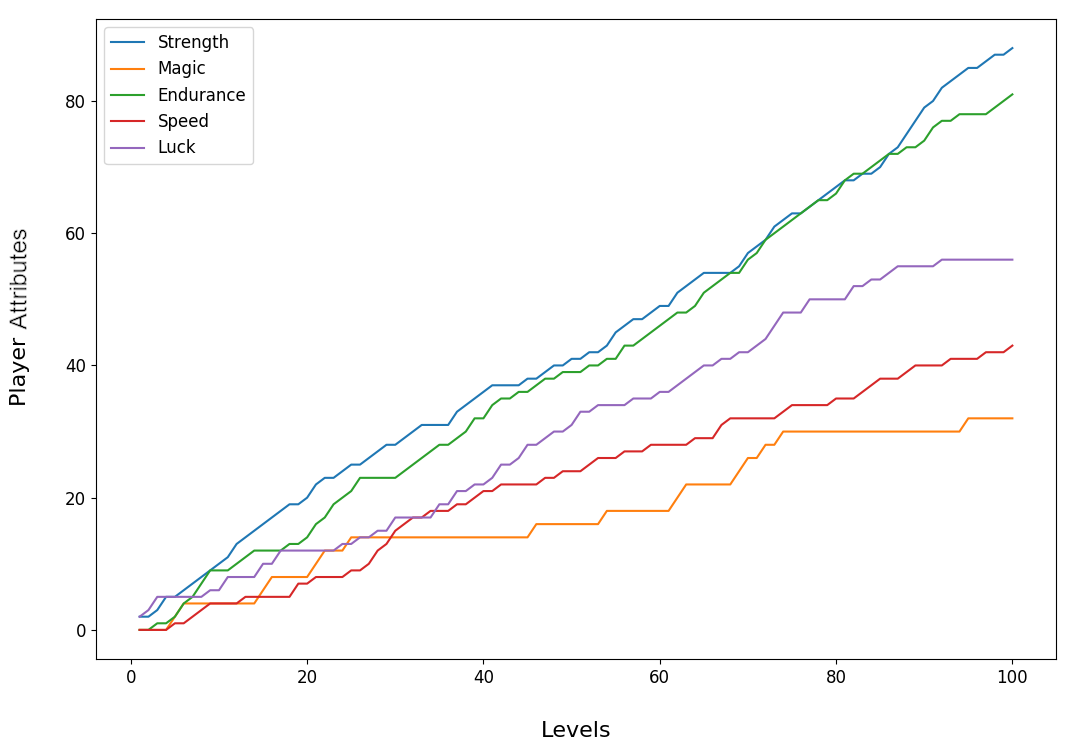
\includegraphics[scale=0.47]{img/PlayerStatsDistrib1.png}
	\caption{Kenaikan atribut \textit{gameplay} karakter pertama pemain setiap levelnya.}
	\label{fig:stats_player_1}
\end{figure}
\vspace{1ex}

\begin{figure} [!h] \centering
	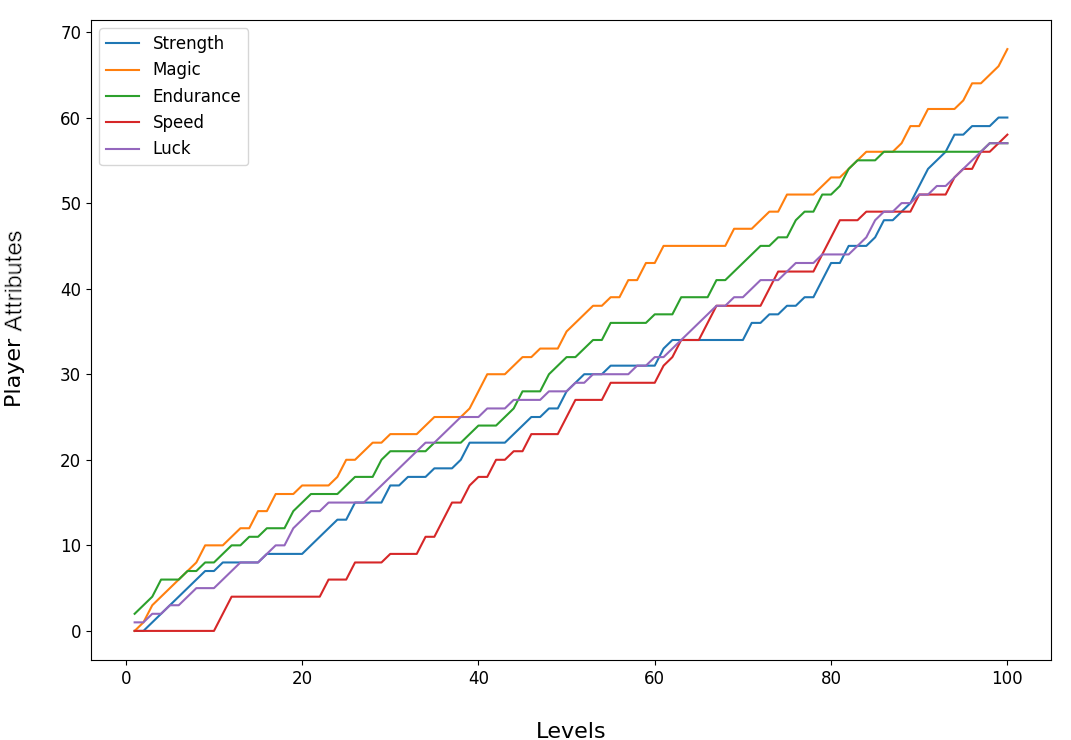
\includegraphics[scale=0.47]{img/PlayerStatsDistrib2.png}
	\caption{Kenaikan atribut \textit{gameplay} karakter kedua pemain setiap levelnya.}
	\label{fig:stats_player_2}
\end{figure}

Pada setiap proses pengujian dalam Sub-bab ini, yang dihasilkan pada Tabel \ref{tb:player_battle_stats} menyajikan sebagian data saja. Hasil selengkapnya dapat dilihat pada Tabel \ref{tb:player_all_stats_1} sampai dengan Tabel \ref{tb:player_all_stats_4} dalam \nameref{chap:chap6_attachment} yang keseluruhan hasil tersebut divisualisasikan pada Gambar \ref{fig:stats_player_1} dan Gambar \ref{fig:stats_player_1}.
\vspace{1ex}

\section{Hasil Atribut Gameplay Musuh}
\label{sec:sec4_eval_turn-based_enemy}
\vspace{1ex}

Pada bagian ini setiap langkah yang akan diuji sudah dijelaskan pada Bagian \ref{sec:sec3_enemy_stats}, dimana pada bagian ini membahas tentang pembuatan atribut \textit{gameplay} musuh untuk permaian dengan genre RPG. Melalui berbagai proses seperti yang dijelaskan pada Bagian \ref{sec:sec3_player_stats}, maka pada beberapa Sub-bab dibawah ini adalah langkah-langkah dalam proses pengujiannya.
\vspace{1ex}


\subsection{Hasil Distibusi Level Musuh}
\label{sec:sub_sec4_eval_dist_enemy_level}
\vspace{1ex}

Seperti yang sudah dijelaskan pada Sub-bab \ref{sec:sub_sec3_enemy_level}, dimana pada bagian ini membahas tentang pendistribusian level musuh untuk permaian dengan genre RPG. Berikut adalah hasil dari proses distribusi level yang diperoleh dari perhitungan pada persamaan \ref{eq:enemy_levels1}, \ref{eq:enemy_levels2}, \ref{eq:sub_enemy_levels1}, \ref{eq:sub_enemy_levels2} dan persamaan \ref{eq:probability_enemy_levels}. Setelah melalui tahapan tersebut dan dengan variabel masukan pada Tabel \ref{tb:enemy_input_variable} maka level yang dihasilkan akan seperti pada Tabel \ref{tb:enemy_level_distrib}.
\vspace{-1ex}

\begin{longtable}{|l|l|l|}
	\caption{Hasil level yang dibuat untuk musuh.}
	\vspace{1ex}
	\label{tb:enemy_level_distrib}\\
	\hline
	\rowcolor[HTML]{C0C0C0} 
	\textbf{No.} & \textbf{Name} & \textbf{Levels} \\ \hline
	1 & Enemy 1 & 1 \\ \hline
	2 & Enemy 2 & 1 \\ \hline
	3 & Enemy 3 & 1 \\ \hline
	4 & Enemy 4 & 1 \\ \hline
	5 & Enemy 5 & 2 \\ \hline
	6 & Enemy 6 & 2 \\ \hline
	7 & Enemy 7 & 2 \\ \hline
	8 & Enemy 8 & 2 \\ \hline
	9 & Enemy 9 & 2 \\ \hline
	10 & Enemy 10 & 2 \\ \hline
	11 & Enemy 11 & 2 \\ \hline
	12 & Enemy 12 & 2 \\ \hline
	13 & Enemy 13 & 2 \\ \hline
	14 & Enemy 14 & 3 \\ \hline
	15 & Enemy 15 & 3 \\ \hline
	... & ... & ... \\ \hline
	\textbf{400} & \textbf{Enemy 400} & \textbf{78} \\ \hline
\end{longtable}
\vspace{1ex}

Pada Tabel \ref{tb:enemy_level_distrib} adalah sebagian data dari level yang dihasilkan oleh program, untuk hasil lebih lengkapnya bisa dilihat pada Tabel \ref{tb:enemy_all_stats_1} sampai Tabel \ref{tb:enemy_all_stats_15} dalam BAB \nameref{chap:chap6_attachment} pada Tabel \ref{tb:enemy_all_stats_1} sampai dengan Tabel \ref{tb:enemy_all_stats_15} di kolom \textit{Levels}. Kemudian persebaran level yang dihasilkan tersebut bila divisualisasikan maka hasilnya akan seperti yang ditujukkkan pada Gambar \ref{fig:enemy_level_distrib}. Grafik atau histogram yang ditunjukan pada Gambar \ref{fig:enemy_level_distrib} tersebut sangatlah tidak merata, hal tersebut dikarenakan proses penentuan level yang ditentukan secara acak.

\begin{figure} [!h] \centering
	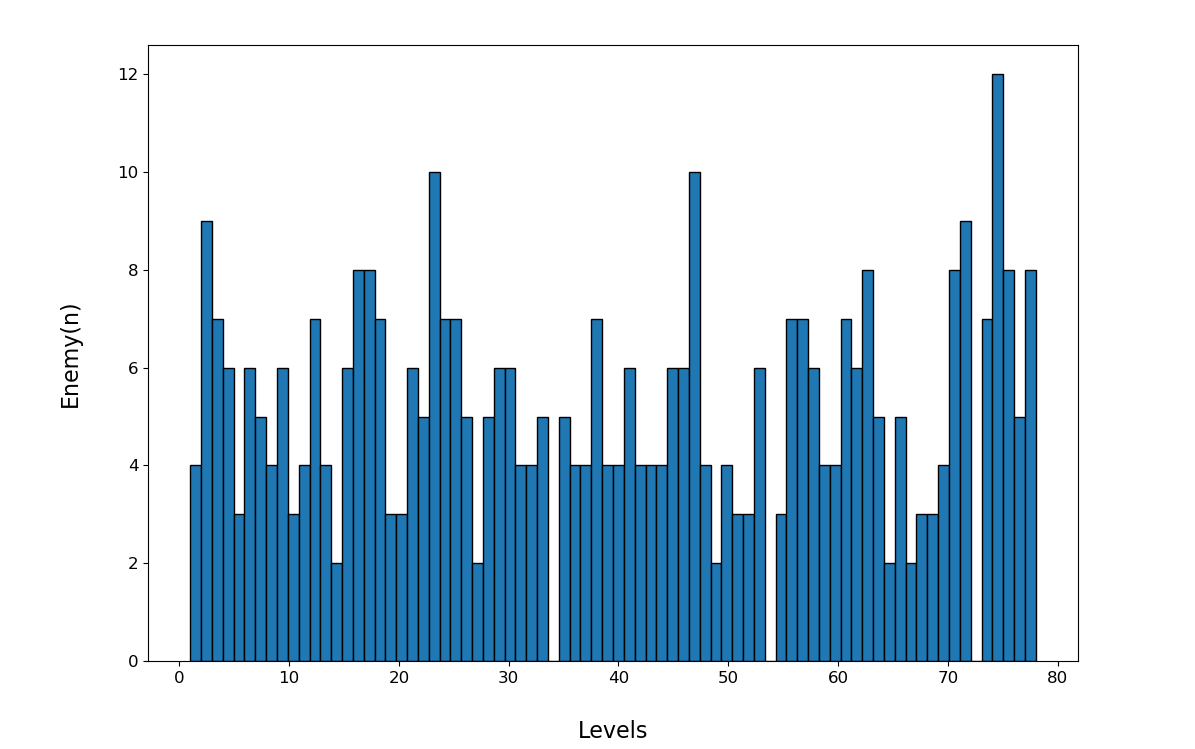
\includegraphics[scale=0.45]{img/EnemyLevelDistrib.png}
	\caption{Distribusi Level Musuh.}
	\label{fig:enemy_level_distrib}
\end{figure}

Di lanjutkan dengan validasi dari keseimbangan persebaran level musuh, hal ini dilakukan dengan menggunakkan persamaan melalui beberapa langkah seperti yang ditunjukan oleh persamaan \ref{eq:mean_enemy_levels}, \ref{eq:varian_enemy_levels}, \ref{eq:stdev_enemy_levels} dan persamaan \ref{eq:PDF_enemy_levels}. Konsep tersebut beracuan pada Sub-bab \ref{sec:sub_sec2_gauss_bayes} tentang \textit{Gaussian Naive bayes}, dengan harapan apakah setiap data yang dihasilkan sebelumnya sudah terdistribusi dengan normal atau tidak. Jika memang benar data hasil program ini valid maka ketika musuh bertambah maka pola dari level dan jumlah musuh masih akan membentuk pola distribusi normal seperti pada Gambar \ref{fig:enemy_level_distrib_ndist}.
\vspace{1ex}

\begin{figure} [!h] \centering
	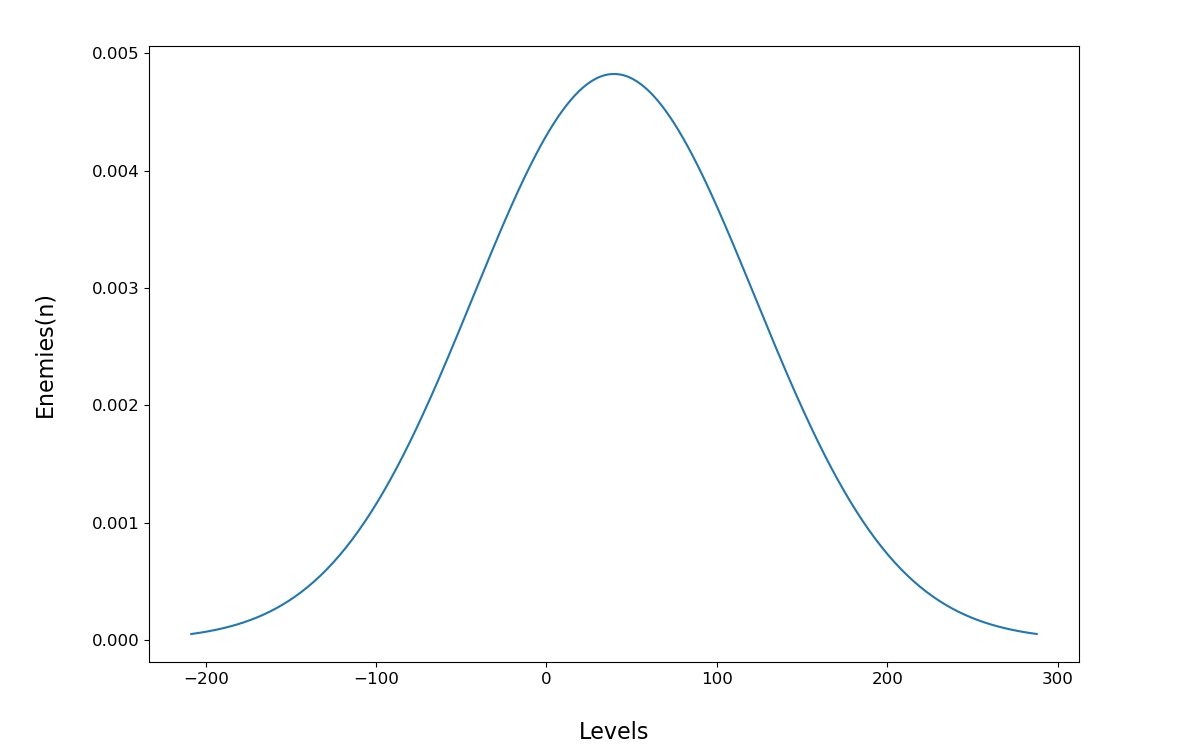
\includegraphics[scale=0.5]{img/EnemyLevelDistribNdist.png}
	\caption{Distribusi level musuh dalam bentuk distribusi normal.}
	\label{fig:enemy_level_distrib_ndist}
\end{figure}

Pada Gambar \ref{fig:enemy_level_distrib_ndist} jika dilihat persebaran datanya dari kiri ke kanan menggambarkan tingkat kesulitan musuh berdasarkan level, jumlah musuh pada sisi kiri berjumlah sedikit semakin ke kanan jumlahnya meningkat dan semakin ke kanan jumlah musuh kembali menjadi sedikit jumlahnya. Hal tersebut menggambarkan tingkat keseimbangan dari musuh yang dibuat, yang mana jumlah musuh dengan level menengah berjumlah paling banyak dan jumlah musuh yang sangat sulit dan sangat mudah dikalahkan berjummlah sedikit. Tujuan utama dari kondisi tersebut adalah terjadinya keseimbangan saat terjadinya pertarungan antara pemain dan musuh.
\vspace{1ex}


\subsection{Hasil Distibusi Tipe Musuh}
\label{sec:sub_sec4_eval_dist_enemy_type}
\vspace{1ex}

Seperti yang sudah dijelaskan pada Sub-bab \ref{sec:sub_sec3_enemy_type}, dimana pada bagian ini membahas tentang pendistribusian tipe musuh untuk permaian dengan genre \textit{turn-based} RPG. Berikut adalah hasil dari proses distribusi tipe musuh yang diperoleh dari perhitungan pada persamaan \ref{eq:enemy_types_percentage}, \ref{eq:enemy_types_dist_level}, \ref{eq:enemy_types_rest_dist_level}, \ref{eq:enemy_types_probability}, \ref{eq:enemy_rest_types} dan persamaan \ref{eq:enemy_types_rest_probability}. Setelah melalui tahapan tersebut dengan variabel masukan pada Tabel \ref{tb:enemy_input_variable} maka hasil distribusi dan penjelasan level yang dilakukan oleh beberapa persamaan tersebut akan menjadi seperti Tabel \ref{tb:enemy_type_distrib}.

\begin{longtable}{|l|l|l|l|}
	\caption{Hasil level yang dibuat untuk musuh.}
	\vspace{1ex}
	\label{tb:enemy_type_distrib}\\
	\hline
	\rowcolor[HTML]{C0C0C0} 
	\textbf{No.} & \textbf{Name} & \textbf{Levels} & \textbf{Type} \\ \hline
	1 & Enemy 1 & 1 & 0 \\ \hline
	2 & Enemy 2 & 1 & 0 \\ \hline
	3 & Enemy 3 & 1 & 2 \\ \hline
	4 & Enemy 4 & 1 & 1 \\ \hline
	5 & Enemy 5 & 2 & 2 \\ \hline
	6 & Enemy 6 & 2 & 1 \\ \hline
	7 & Enemy 7 & 2 & 2 \\ \hline
	8 & Enemy 8 & 2 & 0 \\ \hline
	9 & Enemy 9 & 2 & 2 \\ \hline
	10 & Enemy 10 & 2 & 2 \\ \hline
	11 & Enemy 11 & 2 & 4 \\ \hline
	12 & Enemy 12 & 2 & 0 \\ \hline
	13 & Enemy 13 & 2 & 0 \\ \hline
	14 & Enemy 14 & 3 & 4 \\ \hline
	15 & Enemy 15 & 3 & 4 \\ \hline
	16 & Enemy 16 & 3 & 2 \\ \hline
	... & ... & ... & ... \\ \hline
	\textbf{400} & \textbf{Enemy 400} & \textbf{78} & \textbf{3} \\ \hline
\end{longtable}

Dari data yang tedapat pada Tabel \ref{tb:enemy_type_distrib} hanya sebagian data saja, lebih lengkapnya dapat dilihat langsung pada \nameref{chap:chap6_attachment} dalam Tabel \ref{tb:enemy_all_stats_1} sampai dengan Tabel \ref{tb:enemy_all_stats_15} di kolom \textit{Type}. Pada Tabel \ref{tb:enemy_type_distrib} dan tabel lain yang memuat tentang \textit{Type} yang berisi data $ET_{i}$ atau jenis musuh yang diisi dengan angka 0 sampai dengan 4, maksud dari angka tersebut adalah untuk mewakili indeks dari variabel \textit{Enemy Type} pada Tabel \ref{tb:enemy_input_variable}. Secara berurutan dari 0 sampai dengan 4 adalah \textit{Mixed}, \textit{Hard Magic}, \textit{Soft Magic}, \textit{Hard Strength}, dan \textit{Soft Magic}. Seluruh data tersebut jika divisualisasikan maka hasilnya seperti Gambar \ref{fig:enemy_type_distrib} sesuai yang ditargetkan oleh variabel \textit{Distribute Percentage} pada Tabel \ref{tb:enemy_input_variable} atau variabel $DP$ pada persamaan \ref{eq:enemy_types_percentage}.

\begin{figure} [!h] \centering
	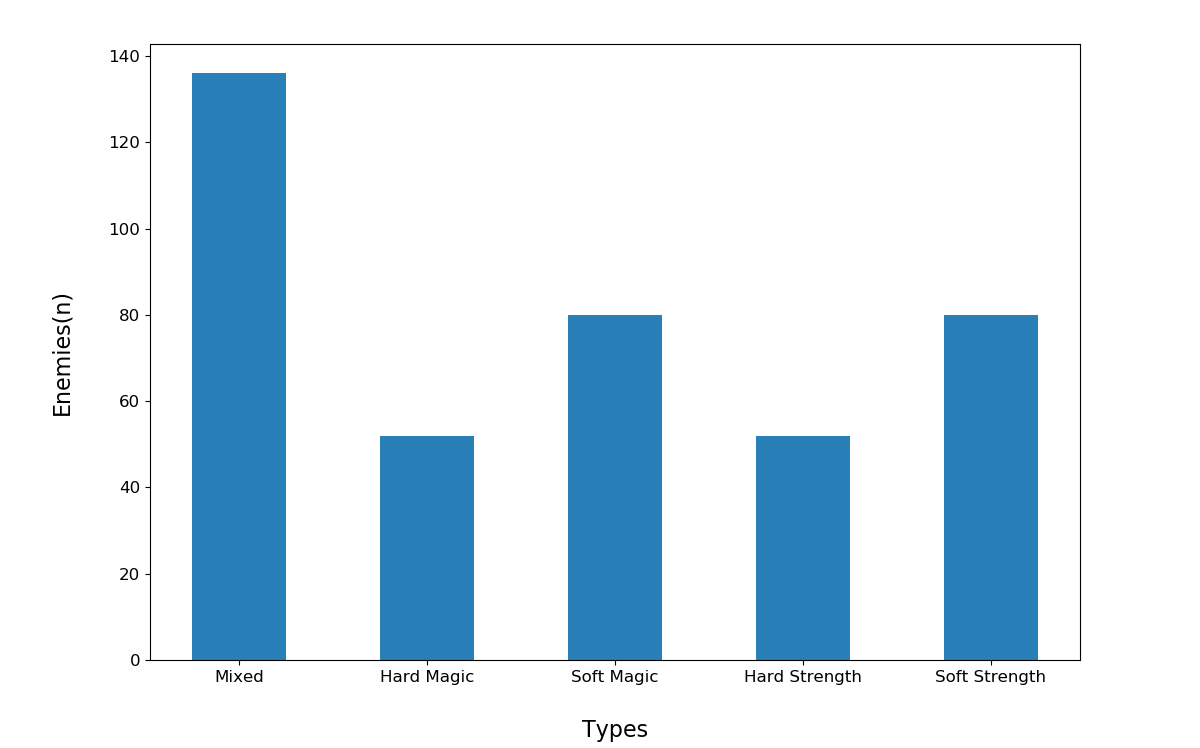
\includegraphics[scale=0.5]{img/EnemyTypeDistrib.png}
	\caption{Distribusi tipe musuh.}
	\label{fig:enemy_type_distrib}
\end{figure}

Kemudian pada Gambar \ref{fig:enemy_type_distrib} adalah hasil dari proses pembuatan dan pengelompokan musuh berdasarkan tipe yang sudah sesuai dengan variabel masukan pada Tabel \ref{tb:enemy_input_variable}. Dengan musuh bertipe \textit{Mixed} berjumlah yang paling banyak, diikuti \textit{soft magic} dan \textit{soft strength} dengan harapan bahwa ini adalah musuh yang memiliki karakter \textit{magic} dan \textit{strength} namun masih mudah dikalahkan, dilanjutkan dengan yang paling sedikit adalah \textit{hard magic} dan \textit{hard strength} dengan harapan menjadi musuh berkarakter strength dan magic yang sulit dikalahkan.
\vspace{1ex}

\subsection{Hasil Distribusi Element dan Kelemahan Musuh}
\label{sec:sub_sec4_eval_dist_enemy_element_and_weak}
\vspace{1ex}

Seperti yang sudah dijelaskan pada Sub-bab \ref{sec:sub_sec3_enemy_weak}, dimana pada bagian ini membahas tentang pendistribusian elemen dan kelemahan musuh untuk permaian dengan genre \textit{turn-based} RPG. Berikut adalah hasil dari proses distribusi tipe musuh yang diperoleh dari perhitungan pada persamaan \ref{eq:enemy_element}, \ref{eq:damage_name_number}, \ref{eq:damage_number_prob}, \ref{eq:multi_damage_num_prob}, dan \ref{eq:all_enemies_damage}. Setelah melalui tahapan tersebut dengan variabel masukan pada Tabel \ref{tb:enemy_input_variable} maka hasil persebaran kelemahan dan kekebalan musuh ditunjukkan pada Tabel \ref{tb:enemy_weak_distrib} dan selengkapnya dapat dilihat pada \nameref{chap:chap6_attachment} dalam Tabel \ref{tb:enemy_all_stats_1} sampai dengan Tabel \ref{tb:enemy_all_stats_15}.
\vspace{-1ex}

\begin{longtable}{|l|l|l|l|l|l|l|}
	\caption{Hasil level yang dibuat untuk musuh.}
	\vspace{1ex}
	\label{tb:enemy_weak_distrib}\\
	\hline
	\rowcolor[HTML]{C0C0C0} 
	\textbf{No.} & \textbf{Name} & \textbf{Phys} & \textbf{Water} & \textbf{Wind} & \textbf{Earth} & \textbf{Fire} \\ \hline
	1 & Enemy 1 & 1 & 1 & 0 & 1 & 0 \\ \hline
	2 & Enemy 2 & 0 & 0 & 0 & 0 & 0 \\ \hline
	3 & Enemy 3 & 0 & 1 & 0 & 1 & 1 \\ \hline
	4 & Enemy 4 & 1 & 0 & 1 & 0 & 0 \\ \hline
	5 & Enemy 5 & 0 & 1 & 0 & 0 & 1 \\ \hline
	6 & Enemy 6 & 1 & 1 & 0 & 1 & 0 \\ \hline
	7 & Enemy 7 & 1 & 0 & 0 & 0 & 0 \\ \hline
	8 & Enemy 8 & 0 & 0 & 0 & 0 & 1 \\ \hline
	9 & Enemy 9 & 1 & 1 & 0 & 0 & 0 \\ \hline
	10 & Enemy 10 & 0 & 0 & 0 & 0 & 0 \\ \hline
	11 & Enemy 11 & 1 & 0 & 0 & 1 & 0 \\ \hline
	12 & Enemy 12 & 0 & 0 & 0 & 0 & 1 \\ \hline
	13 & Enemy 13 & 0 & 0 & 2 & 1 & 0 \\ \hline
	%14 & Enemy 14 & 0 & 1 & 0 & 0 & 0 \\ \hline
	... & ... & ... & ... & ... & ... & ... \\ \hline
	\textbf{400} & \textbf{Enemy 400} & \textbf{0} & \textbf{0} & \textbf{2} & \textbf{1} & \textbf{0} \\ \hline
\end{longtable}
\vspace{1ex}

Jika melihat Tabel \ref{tb:enemy_weak_distrib} dengan melihat pada kolom \textit{Phys}, \textit{Water}, \textit{Wind}, \textit{Earth}, dan \textit{Fire}, isi dari kolom tersebut berupa angka nol sampai dengan dua adalah hasil dari pembuatan atribut \textit{gameplay} kelemahan musuh pada variabel $DmgEN_{M} = \left \{ DmgNu_{0}, DmgNu_{1}, DmgNu_{2}, ..., DmgNu_{M} \right \}$ jika jumlah kelemahan musuh lebih dari tiga atau yang dicontohkan pada Tabel \ref{tb:enemy_input_variable} dalam variabel \textit{List Damage}. Hasil dari proses yang sebelumnya dijelaskan pada Sub-bab ini menghasilkan persebaran kelemahan dan kekebalan musuh yang ditunjukkan pada Gambar \ref{fig:enemy_weak_distrib} dibawah ini.

\begin{figure} [!h] \centering
	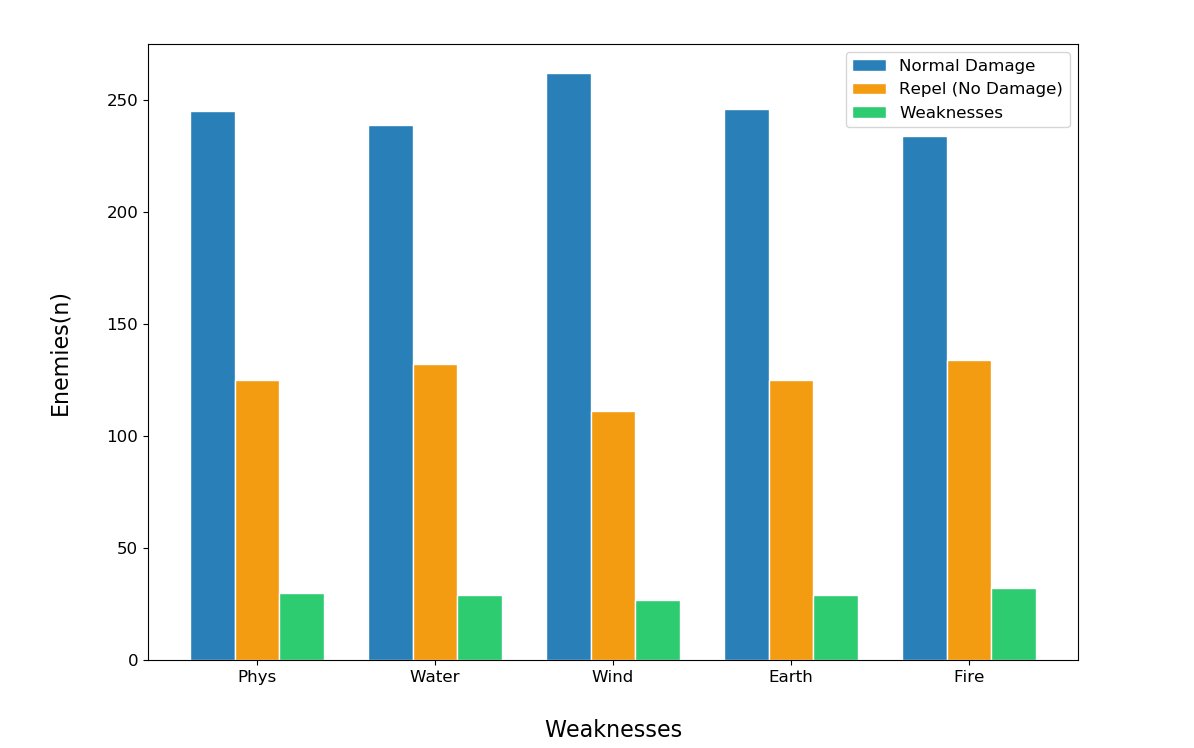
\includegraphics[scale=0.50]{img/EnemyWeakDistrib.png}
	\caption{Distribusi kelemahan musuh.}
	\label{fig:enemy_weak_distrib}
\end{figure}

Pada Gambar \ref{fig:enemy_weak_distrib} dapat dilihat distribusi musuh dengan kelemahan dan kekebalannya. Terlihat pada kondisi tersebut jumlah musuh dengan kondisi \textit{Normal} memiliki nilai paling tunggi pada setiap kelemahan, hal tersebut dapat diartikan bahwa sebagian besar elemen dari musuh dapat memperoleh \textit{damage} secara normal jika diserang. Kemudian jumlah musuh pada kondisi \textit{Repel} berjumlah terbanyak kedua, hal tersebut dapat diartikan musuh memmiliki jumlah kekebalan terhadap serangan sejumlah angka pada setiap elemen pada Gambar \ref{fig:enemy_weak_distrib}. Begitu juga dengan kondisi \textit{Weaknesses} dengan jumlah paling sedikit, hal tersebut bertujuan agar menjadikan pertarungan antara pemain dan musuh menjadi tidak mudah dimenangkan oleh pemain. Tidak hanya dengan efek \textit{Weaknesses}, efek \textit{Repel} juga sangat berpengaruh dalam menjadikan permainan seperti layaknya sebuah \textit{puzzle} atau teka-teki.
\vspace{1ex}

Sedangkan pada persamaan \ref{eq:multi_damage_num_prob} adalah penjelasan tentang proses munculnya setiap $DmgNu$ pada satu karakter musuh, sehingga variabel tersebut berubah menjadi $DmgNu_{i}$. Seperti penjelasan sebelumnya bahwa pada sebuah karakter musuh dapat memiliki lebih dari satu kelemahan atau kekebalan $DmgNu$ terhadap $DmgNa$ yang diset secara acak seperti yang sudah dijelaskan pada bagian sebelumnya. 
\vspace{1ex}

\subsection{Hasil Distribusi HP, MP, dan Atribut Gameplay pada Musuh}
\label{sec:sub_sec4_eval_dist_enemy_HP_MP_Stats}
\vspace{1ex}

pada Sub-bab \ref{sec:sub_sec3_enemy_hp_mp_stats}, dimana pada bagian ini membahas tentang pendistribusian HP dan MP musuh untuk permaian dengan genre \textit{turn-based} RPG. Berikut adalah hasil dari proses distribusi tipe musuh yang diperoleh dari perhitungan pada persamaan \ref{eq:enemy_types_stats_ex} sampai dengan persamaan \ref{eq:enemy_types_prob_hp_mix}, yang mana pada persamaan \ref{eq:enemy_types_stats_ex} sampai dengan persamaan \ref{eq:enemy_types_prob_adv} adalah penenentuan tipe musuh. Setelah melalui tahapan tersebut dengan variabel masukan pada Tabel \ref{tb:enemy_input_variable} maka hasil persebaran kelemahan dan kekebalan musuh ditunjukkan pada Tabel \ref{tb:enemy_weak_distrib}.
\vspace{-1ex}

\begin{longtable}{|l|l|l|l|l|}
	\caption{Distribusi atribut \textit{gameplay} HP dan MP musuh.}
	\vspace{1ex}
	\label{tb:enemy_weak_stats}\\
	\hline
	\rowcolor[HTML]{C0C0C0} 
	\textbf{No.} & \textbf{Name} & \textbf{Levels} & \textbf{HP} & \textbf{MP} \\ \hline
	1 & Enemy 1 & 1 & 42 & 45 \\ \hline
	2 & Enemy 2 & 1 & 84 & 21 \\ \hline
	3 & Enemy 3 & 1 & 43 & 51 \\ \hline
	4 & Enemy 4 & 1 & 44 & 231 \\ \hline
	5 & Enemy 5 & 2 & 40 & 40 \\ \hline
	6 & Enemy 6 & 2 & 44 & 208 \\ \hline
	7 & Enemy 7 & 2 & 44 & 47 \\ \hline
	8 & Enemy 8 & 2 & 42 & 53 \\ \hline
	9 & Enemy 9 & 2 & 49 & 53 \\ \hline
	10 & Enemy 10 & 2 & 42 & 49 \\ \hline
	11 & Enemy 11 & 2 & 44 & 23 \\ \hline
	12 & Enemy 12 & 2 & 79 & 27 \\ \hline
	13 & Enemy 13 & 2 & 41 & 26 \\ \hline
	14 & Enemy 14 & 3 & 50 & 34 \\ \hline
	15 & Enemy 15 & 3 & 54 & 20 \\ \hline
	... & ... & ... & ... & ... \\ \hline
	\textbf{400} & \textbf{Enemy 400} & \textbf{78} & \textbf{389} & \textbf{161} \\ \hline
\end{longtable}
\vspace{1ex}

Pada Tabel \ref{tb:enemy_weak_stats} hanya sebagian data saja yang ditampilkan, untuk selengkapnya dapat dilihat pada \nameref{chap:chap6_attachment} dalam Tabel \ref{tb:enemy_all_stats_1} sampai dengan Tabel \ref{tb:enemy_all_stats_15} pada kolom HP dan MP. Selanjutnya adalah penggambaran persebaran HP dan MP yang masing-masing digambarkan pada Gambar \ref{fig:enemy_hp_distrib} dan Gambar \ref{fig:enemy_mp_distrib}.
\vspace{1ex}

\begin{figure} [!h] \centering
	\centering
	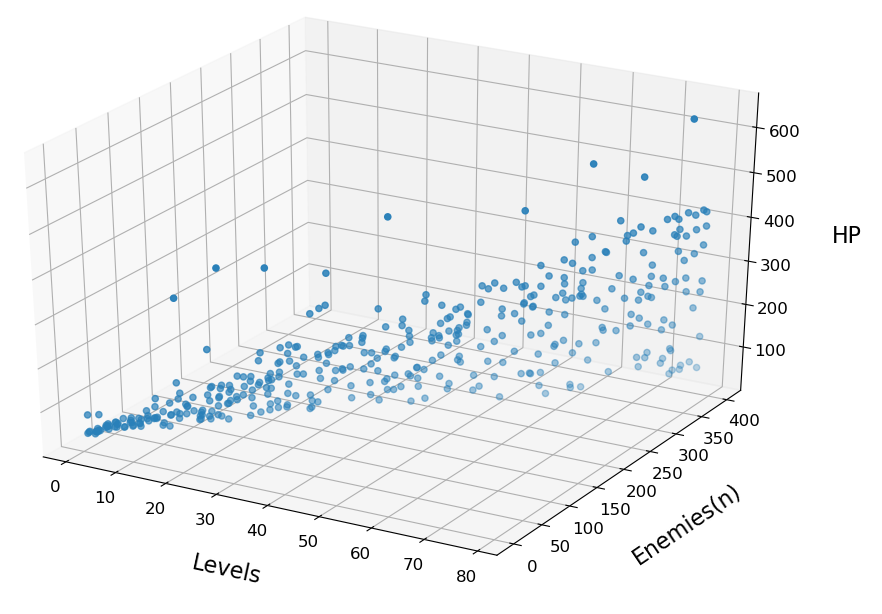
\includegraphics[scale=0.52]{img/EnemyHpDistrib.png}
	\caption{Distribusi atribut \textit{gameplay} HP musuh.}
	\label{fig:enemy_hp_distrib}
\end{figure}

\begin{figure} [!h] \centering
	\centering
	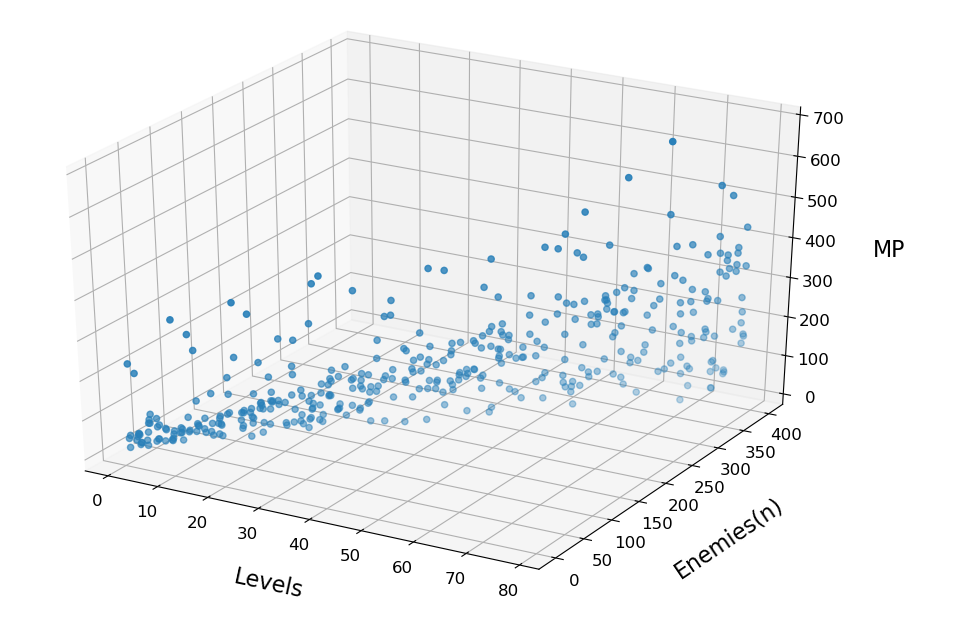
\includegraphics[scale=0.52]{img/EnemyMpDistrib.png}
	\caption{Distribusi atribut \textit{gameplay} MP musuh.}
	\label{fig:enemy_mp_distrib}
\end{figure}
\vspace{1ex}

Masih pada Sub-bab \ref{sec:sub_sec3_enemy_hp_mp_stats}, dimana pada bagian ini membahas tentang pendistribusian atribut \textit{gameplay} musuh untuk permaian dengan genre \textit{turn-based} RPG. Berikut adalah hasil dari proses distribusi tipe musuh yang diperoleh dari perhitungan mulai dari persamaan \ref{eq:enemy_types_stats_ex} secara berurutan sampai dengan persamaan \ref{eq:enemy_types_prob_adv} yang digunakan untuk penentuan tipe musuh yang ingin dipakai. 
\vspace{1ex}

Sedangkan proses kalkulasi untuk menentukan atribut \textit{gameplay} musuh dimulai dari persamaan \ref{eq:enemy_types_prob_bst1} sampai dengan persamaan \ref{eq:enemy_types_prob_st}. Setelah melalui tahapan tersebut dengan variabel masukan pada Tabel \ref{tb:enemy_input_variable} maka hasil persebaran atribut \textit{gameplay} musuh dengan komposisi \textit{Strength}, \textit{Magic}, \textit{Endurance}, \textit{Speed}, dan \textit{Luck} ditunjukkan pada Tabel \ref{tb:enemy_stats}.
\vspace{-1ex}

\begin{longtable}{|l|l|l|l|l|l|l|l|}
	\caption{Distribusi atribut \textit{gameplay} musuh.}
	\vspace{1ex}
	\label{tb:enemy_stats}\\
	\hline
	\rowcolor[HTML]{C0C0C0} 
	\textbf{No.} & \textbf{Name} & \textbf{Lv.} & \textbf{Str} & \textbf{Mag} & \textbf{Endr} & \textbf{Spd} & \textbf{Luck} \\ \hline
	1 & Enemy 1 & 1 & 2 & 2 & 2 & 2 & 2 \\ \hline
	2 & Enemy 2 & 1 & 2 & 2 & 2 & 2 & 2 \\ \hline
	3 & Enemy 3 & 1 & 2 & 2 & 6 & 2 & 2 \\ \hline
	4 & Enemy 4 & 1 & 2 & 2 & 6 & 2 & 2 \\ \hline
	5 & Enemy 5 & 2 & 2 & 3 & 6 & 3 & 2 \\ \hline
	6 & Enemy 6 & 2 & 2 & 3 & 9 & 2 & 2 \\ \hline
	7 & Enemy 7 & 2 & 2 & 3 & 6 & 2 & 2 \\ \hline
	8 & Enemy 8 & 2 & 2 & 3 & 2 & 2 & 2 \\ \hline
	9 & Enemy 9 & 2 & 2 & 3 & 10 & 3 & 2 \\ \hline
	10 & Enemy 10 & 2 & 2 & 3 & 11 & 3 & 2 \\ \hline
	11 & Enemy 11 & 2 & 2 & 3 & 2 & 2 & 2 \\ \hline
	12 & Enemy 12 & 2 & 2 & 3 & 12 & 3 & 2 \\ \hline
	13 & Enemy 13 & 2 & 2 & 3 & 6 & 2 & 2 \\ \hline
	14 & Enemy 14 & 3 & 2 & 8 & 2 & 2 & 2 \\ \hline
	15 & Enemy 15 & 3 & 3 & 11 & 2 & 3 & 2 \\ \hline
	16 & Enemy 16 & 3 & 2 & 2 & 11 & 2 & 2 \\ \hline
	... & ... & ... & ... & ... & ... & ... & ... \\ \hline
	\textbf{400} & \textbf{Enemy 400} & \textbf{78} & \textbf{30} & \textbf{15} & \textbf{11} & \textbf{36} & \textbf{22} \\ \hline
\end{longtable}
\vspace{1ex}

Selanjutnya adalah penggambaran persebaran atribut \textit{gameplay} yang disebutkan pada Tabel \ref{tb:enemy_stats} yang digambarkan pada Gambar \ref{fig:enemy_stats_distrib}. Pada Gambar \ref{fig:enemy_str_distrib}, \ref{fig:enemy_mag_distrib}, \ref{fig:enemy_endr_distrib}, \ref{fig:enemy_spd_distrib} dan Gambar \ref{fig:enemy_luck_distrib} adalah pecahan dari Gambar \ref{fig:enemy_stats_distrib} secara berurutan diantaranya adalah \textit{Strength}, \textit{Magic}, \textit{Endurance}, \textit{Speed} dan \textit{Luck}. Data atribut \textit{gameplay} selengkapnya dapat dilihat pada \nameref{chap:chap6_attachment} dalam Tabel \ref{tb:enemy_all_stats_1} sampai dengan Tabel \ref{tb:enemy_all_stats_15} pada kolom \textit{Strength}, \textit{Magic}, \textit{Endurance}, \textit{Speed}, \textit{Luck} dan atribut \textit{gameplay} yang lain jika dilakukan penambahan atribut \textit{gameplay} pada program. 
\clearpage

\begin{figure} [!h] \centering
	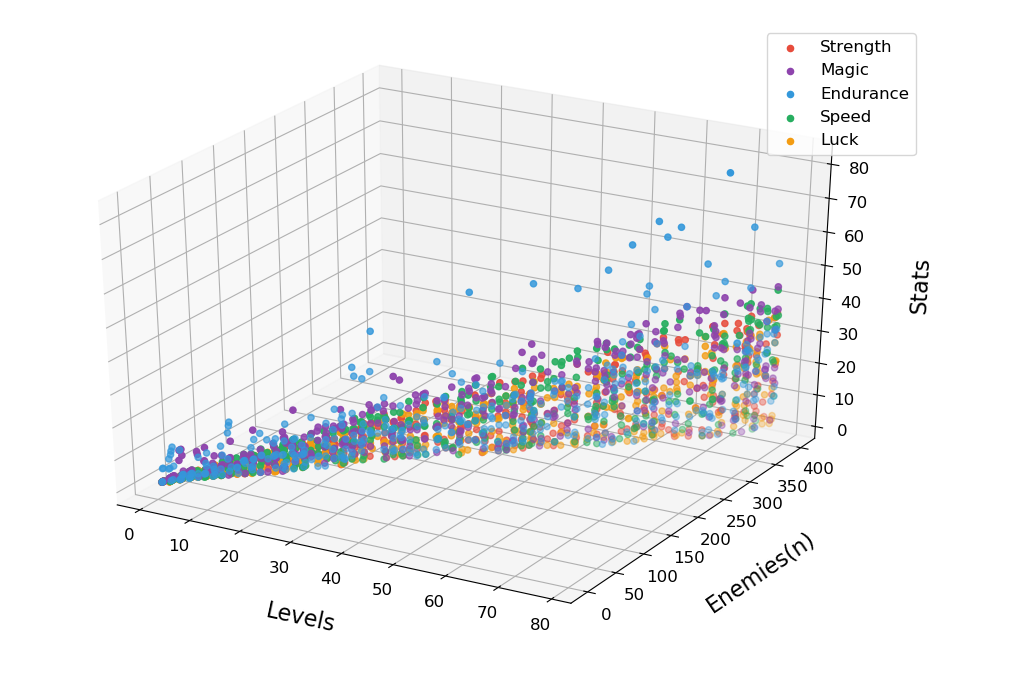
\includegraphics[scale=0.6]{img/EnemyStatsDistrib.png}
	\caption{Distribusi atribut \textit{gameplay} musuh secara keseluruhan.}
	\label{fig:enemy_stats_distrib}
	\vspace{5ex}

	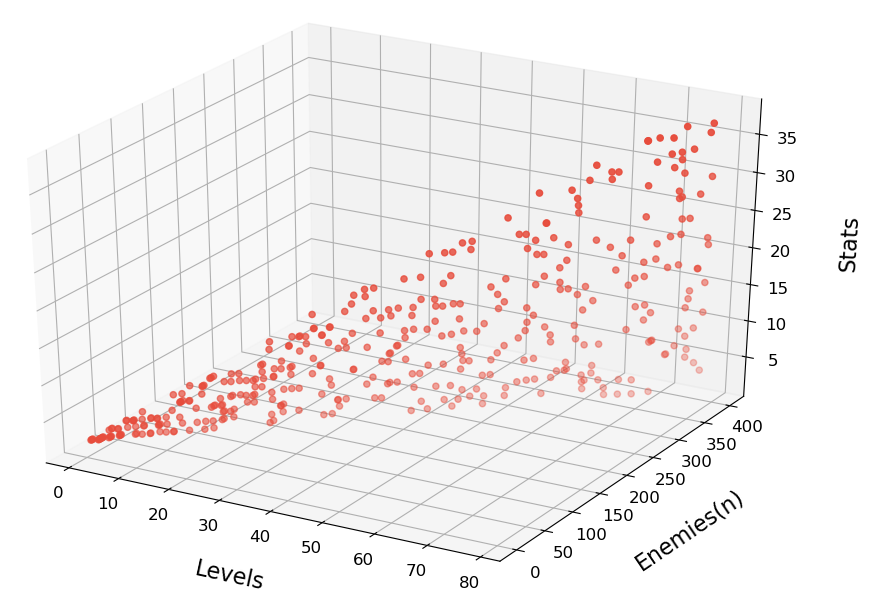
\includegraphics[scale=0.6]{img/EnemyStrengthDistrib.png}
	\caption{Distribusi \textit{Strength} musuh.}
	\label{fig:enemy_str_distrib}
\end{figure}
\clearpage

\begin{figure} [!h] \centering
	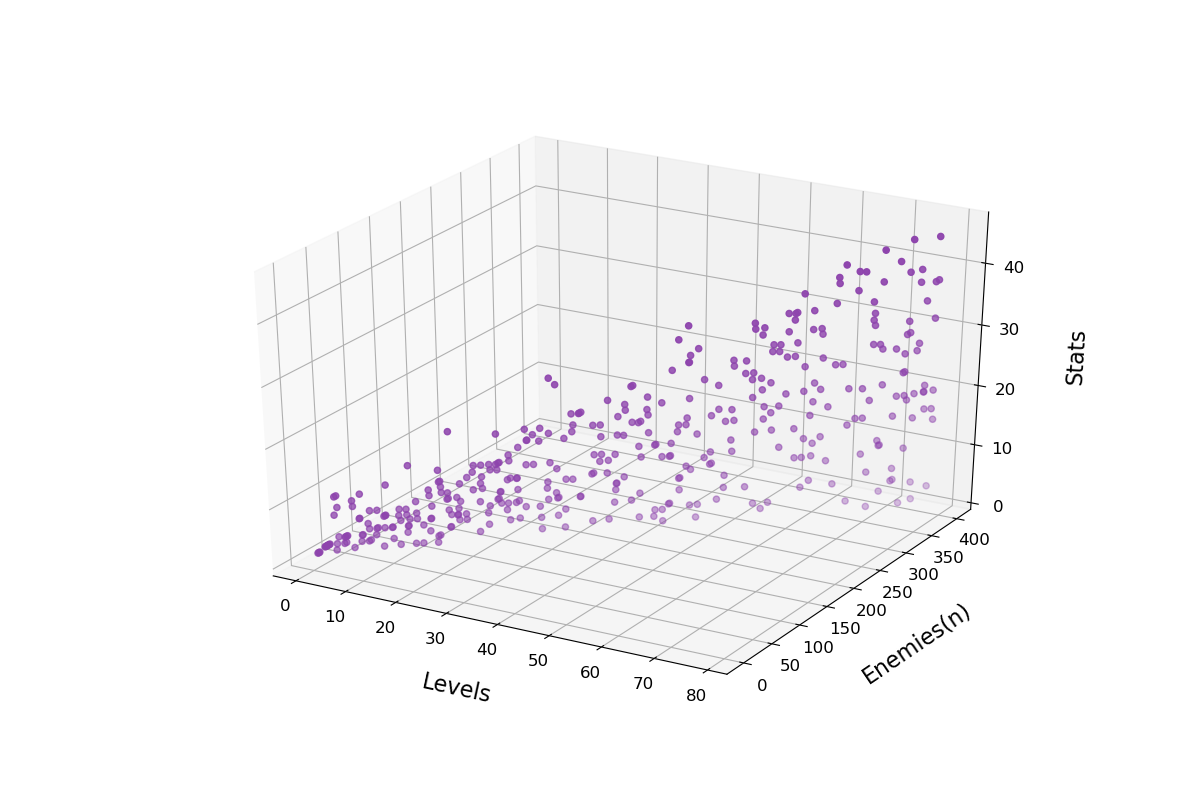
\includegraphics[scale=0.6]{img/EnemyMagicDistrib.png}
	\caption{Distribusi \textit{Magic} musuh.}
	\label{fig:enemy_mag_distrib}
	\vspace{5ex}

	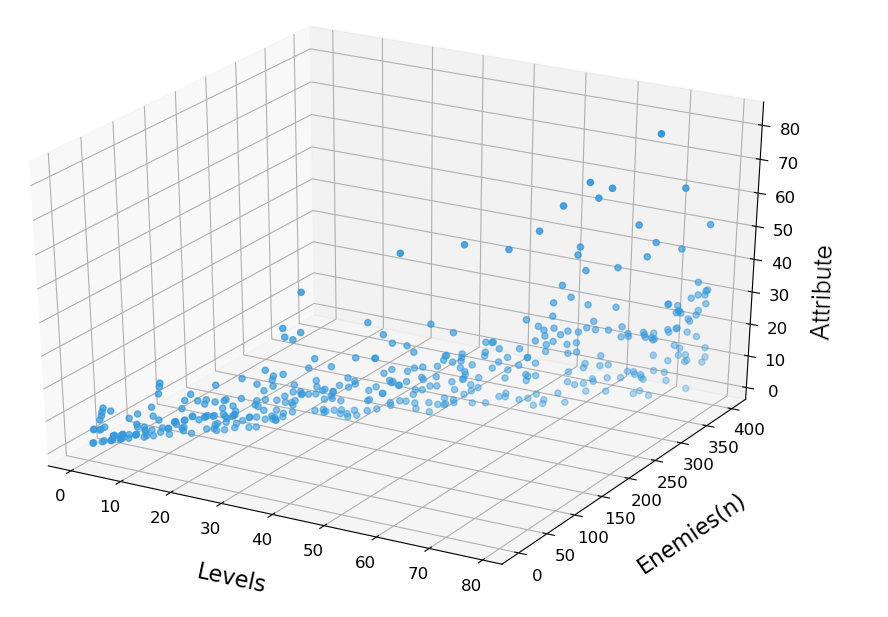
\includegraphics[scale=0.6]{img/EnemyEnduranceDistrib.png}
	\caption{Distribusi \textit{Endurance} musuh.}
	\label{fig:enemy_endr_distrib}
\end{figure}

\begin{figure} [!h] \centering
	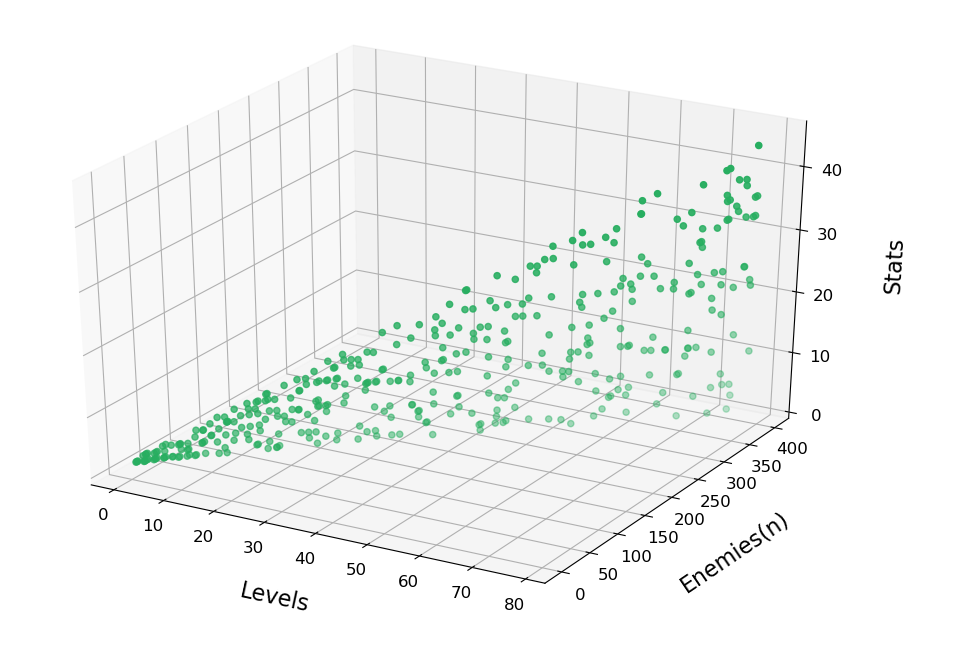
\includegraphics[scale=0.6]{img/EnemySpeedDistrib.png}
	\caption{Distribusi \textit{Speed} musuh.}
	\label{fig:enemy_spd_distrib}
	\vspace{5ex}

	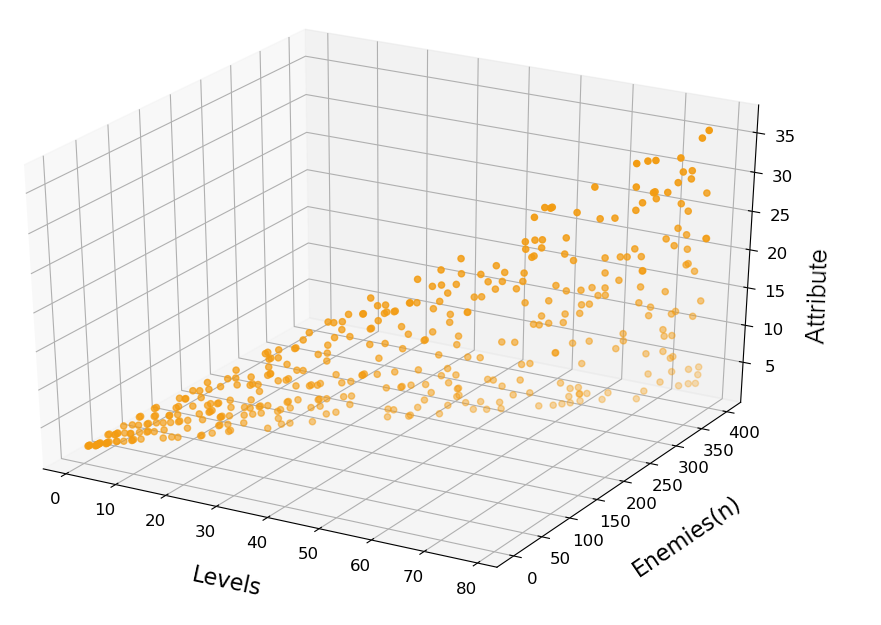
\includegraphics[scale=0.6]{img/EnemyLuckDistrib.png}
	\caption{Distribusi \textit{Luck} musuh.}
	\label{fig:enemy_luck_distrib}
\end{figure}
\clearpage

\section{Hasil Klasifikasi Karakter pada Permainan Dota 2}
\label{sec:sec4_eval_dota2}
\vspace{1ex}

Pada Sub-bab ini akan membahas hasil dari Sub-bab \ref{sec:sec3_dota2_method}, bila dijelaskan melalui diagram blok pada Gambar \ref{fig:dota2_class_proc} maka bagian yang akan dibahas pada Sub-bab ini adalah proses saat klasifikasi. Grafik hasil \textit{training} dapat dilihat pada Gambar \ref{fig:nn_dota2_acc_chap4}, \ref{fig:nn_dota2_loss_chap4}, \ref{fig:nn_dota2_lr_chap4}, \ref{fig:nn_dota2_val_acc_chap4}, dan Gambar \ref{fig:nn_dota2_val_loss_chap4}. Masing-masing Gambar tersebut secara berurutan adalah akurasi saat \textit{training}, \textit{loss} saat \textit{training}, \textit{learning rate} saat \textit{training}, akurasi saat evaluasi dan \textit{loss} saat evaluasi. 
\vspace{2ex}

\begin{figure} [!h] \centering
	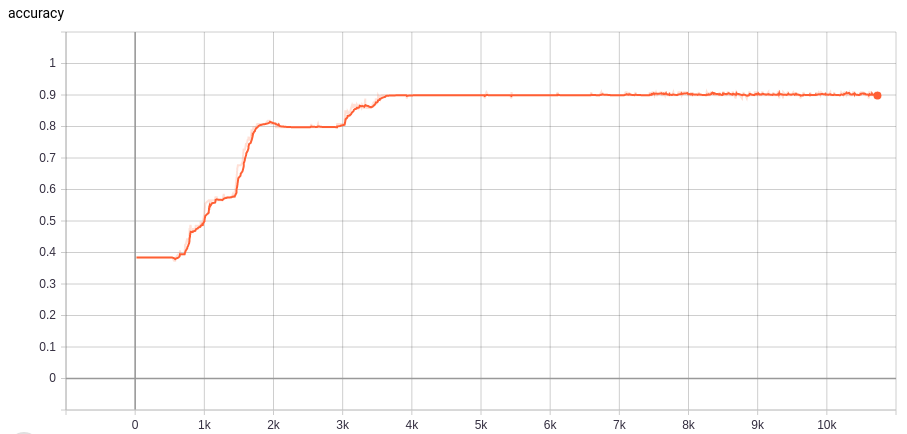
\includegraphics[scale=0.44]{img/callback_acc_chap4.png}
	\caption{Akurasi saat \textit{training} pada \textit{hero} Dota 2.}
	\label{fig:nn_dota2_acc_chap4}
	\vspace{4ex}

	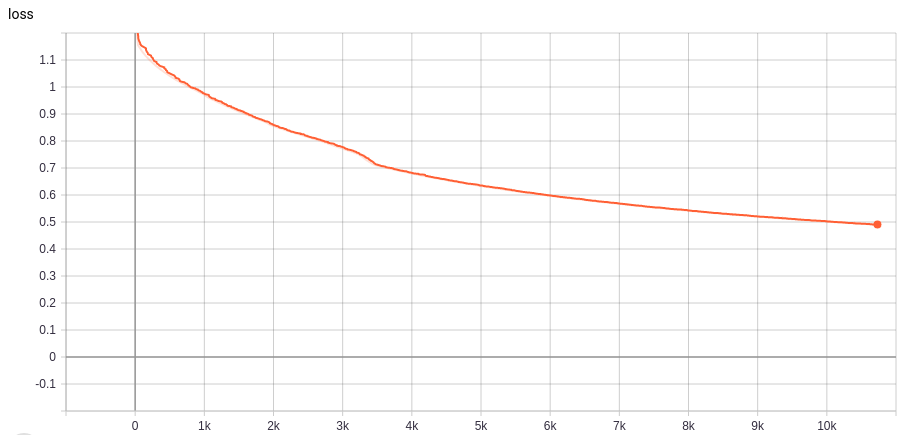
\includegraphics[scale=0.44]{img/callback_loss_chap4.png}
	\caption{\textit{Loss} saat \textit{training} pada \textit{hero} Dota 2.}
	\label{fig:nn_dota2_loss_chap4}
\end{figure}
\clearpage

\begin{figure} [!h] \centering
	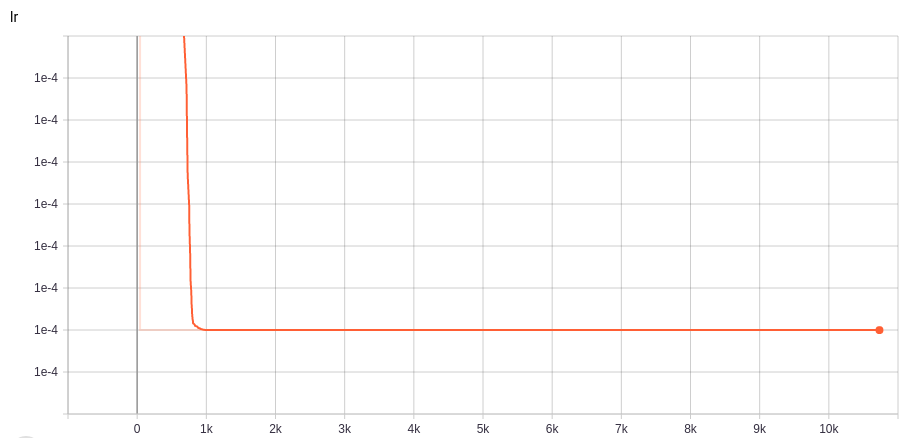
\includegraphics[scale=0.4]{img/callback_lr_chap4.png}
	\caption{\textit{Learning rate} saat \textit{training} pada \textit{hero} Dota 2.}
	\label{fig:nn_dota2_lr_chap4}
	\vspace{4ex}

	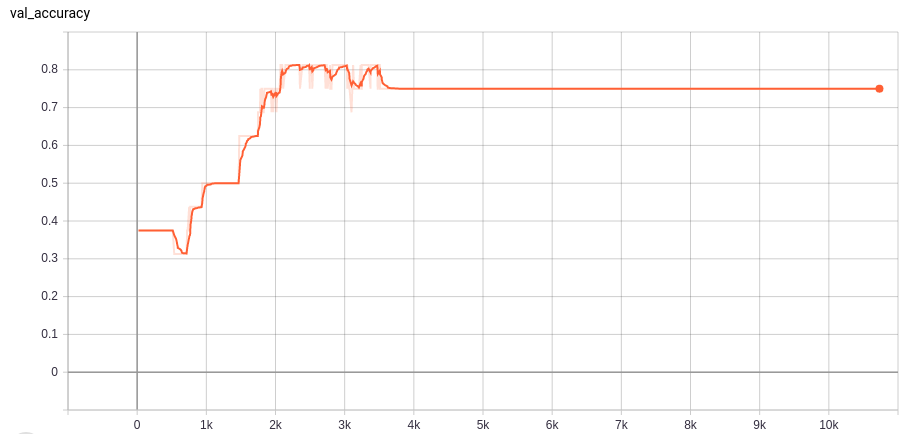
\includegraphics[scale=0.4]{img/callback_val_acc_chap4.png}
	\caption{Akurasi pada saat proses evaluasi pada \textit{hero} Dota 2.}
	\label{fig:nn_dota2_val_acc_chap4}
	\vspace{4ex}

	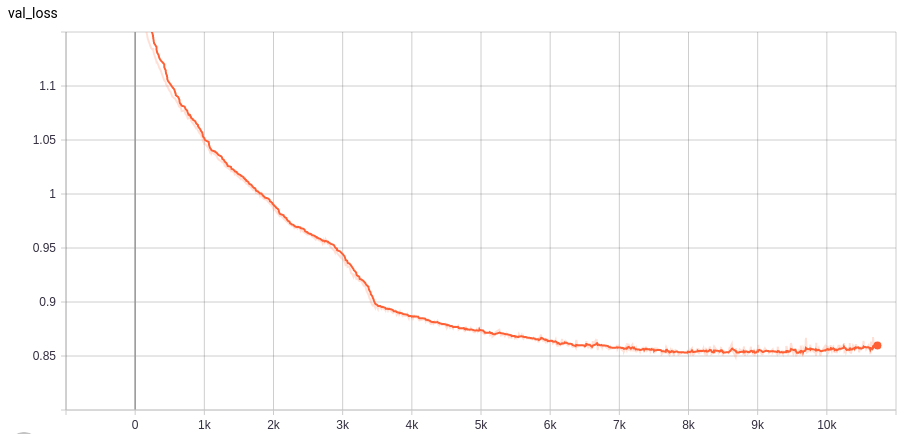
\includegraphics[scale=0.4]{img/callback_val_loss_chap4.png}
	\caption{\textit{Loss} saat proses evaluasi pada \textit{hero} Dota 2.}
	\label{fig:nn_dota2_val_loss_chap4}
\end{figure}
\clearpage

Seperti penjelasan tentang proses \textit{training} pada Sub-bab \ref{sec:sub_sec3_dota2_train}, \textit{training} berlangsung selama 10.730 \textit{epoch}. Akurasi saat \textit{training} mampu mencapai 0.9 dan mengalami \textit{loss} sebesar 0.55, kemudian akurasi saat evaluasi mampu mencapai 0.75 dan mengalami \textit{loss} saat evaluasi sebesar 0.86 . Hasil klasifikasi dari data atribut \textit{gameplay} karakter atau \textit{hero} Dota 2 yang dijadikan sebagai data \textit{testing} dapat dilihat pada Tabel \ref{tb:dota2_hero_pt3} yang kemudian digunakan pada proses evalusi dan \textit{testing} dengan hasil yang ditampilkan pada Tabel \ref{tb:dota2_valid_result}.
\vspace{-2ex}

\begin{longtable}{|l|l|l|l|}
	\caption{Hasil proses \textit{testing} dengan data \textit{testing} pada \textit{hero} Dota 2.}
	\vspace{1ex}
	\label{tb:dota2_valid_result}\\
	\hline
	\rowcolor[HTML]{C0C0C0} 
	\textbf{Hero Name} & \textbf{Strength} & \textbf{Agility} & \textbf{Intelligent} \\ \hline
	\rowcolor[HTML]{FFFFFF} 
	\textbf{ArcWarden} & 0.053558 & 0.206808 & {\color[HTML]{FE0000} 0.739634} \\ \hline
	\rowcolor[HTML]{FFFFFF} 
	\textbf{Jakiro} & 0.205992 & 0.241550 & {\color[HTML]{036400} 0.552458} \\ \hline
	\rowcolor[HTML]{FFFFFF} 
	\textbf{WinterWyvern} & 0.205992 & 0.241552 & {\color[HTML]{036400} 0.552456} \\ \hline
	\rowcolor[HTML]{FFFFFF} 
	\textbf{Bloodseeker} & 0.161604 & {\color[HTML]{036400} 0.760779} & 0.077617 \\ \hline
	\rowcolor[HTML]{FFFFFF}
	\textbf{Phoenix} & 0.053562 & 0.206812 & {\color[HTML]{FE0000} 0.739627} \\ \hline
	\rowcolor[HTML]{FFFFFF} 
	\textbf{Io} & 0.053558 & 0.206813 & {\color[HTML]{FE0000} 0.739629} \\ \hline
	\rowcolor[HTML]{FFFFFF} 
	\textbf{Leshrac} & 0.053559 & 0.206871 & {\color[HTML]{036400} 0.739570} \\ \hline
	\rowcolor[HTML]{FFFFFF} 
	\textbf{OutworldDevourer} & 0.205848 & 0.245712 & {\color[HTML]{036400} 0.548440} \\ \hline
	\rowcolor[HTML]{FFFFFF} 
	\textbf{Brewmaster} & {\color[HTML]{036400} 0.624197} & 0.189504 & 0.186300 \\ \hline
	\rowcolor[HTML]{FFFFFF} 
	\textbf{Tusk} & 0.377984 & {\color[HTML]{FE0000} 0.510914} & 0.111102 \\ \hline
	\rowcolor[HTML]{FFFFFF} 
	\textbf{Weaver} & 0.098899 & {\color[HTML]{036400} 0.560487} & 0.340614 \\ \hline
	\rowcolor[HTML]{FFFFFF} 
	\textbf{Undying} & {\color[HTML]{036400} 0.645770} & 0.127254 & 0.226976 \\ \hline
	\rowcolor[HTML]{FFFFFF} 
	\textbf{Alchemist} & {\color[HTML]{036400} 0.643663} & 0.126769 & 0.229569 \\ \hline
	\rowcolor[HTML]{FFFFFF} 
	\textbf{Phantom Lancer} & 0.154832 & {\color[HTML]{036400} 0.768835} & 0.076333 \\ \hline
	\rowcolor[HTML]{FFFFFF} 
	\textbf{CrystalMaiden} & 0.053558 & 0.206809 & {\color[HTML]{036400} 0.739633} \\ \hline
	\rowcolor[HTML]{FFFFFF} 
	\textbf{Invoker} & 0.053558 & 0.206809 & {\color[HTML]{036400} 0.739633} \\ \hline
\end{longtable}

Cara membaca hasil klasifikasi pada Tabel \ref{tb:dota2_valid_result} sebelumnya sudah dijelaskan pada Sub-bab \ref{sec:sub_sec3_dota2_arch} dan Sub-bab \ref{sec:sub_sec3_dota2_train}. Hasil ditampilkan pada Tabel \ref{tb:dota2_valid_result} terdapat 4 \textit{hero} yang mengalami salah klasifikasi yang kemudian diberi warna merah, dengan beracuan pada kolom \textit{type} dalam Tabel \ref{tb:dota2_hero_pt3} yang terlampir pada \nameref{chap:chap6_attachment}. Maka dari 16 \textit{hero} terdapat 4 hero yang mengalami salah klasifikasi, jadi presentasenya 64\% \textit{hero} berhasil terklasifikasi.
\vspace{1ex}

\section{Hasil Klasifikasi Karakter Pemain}
\label{sec:sec4_eval_player}
\vspace{1ex}

Pada Sub-bab ini akan membahas hasil dari Sub-bab \ref{sec:sec3_player_method}, bila dijelaskan melalui diagram blok pada Gambar \ref{fig:player_class_proc} maka bagian yang akan dibahas pada Sub-bab ini adalah klasifikasi. Grafik hasil \textit{training} dapat dilihat pada Gambar \ref{fig:nn_player_acc_chap4}, \ref{fig:nn_player_loss_chap4}, \ref{fig:nn_player_lr_chap4}, \ref{fig:nn_player_val_acc_chap4}, dan Gambar \ref{fig:nn_player_val_loss_chap4}. Masing-masing dari Gambar tersebut secara berurutan adalah akurasi saat \textit{training}, \textit{loss} saat \textit{training}, \textit{learning rate} saat \textit{training}, akurasi saat evaluasi dan \textit{loss} saat evaluasi.
\vspace{2ex}

\begin{figure} [!h] \centering
	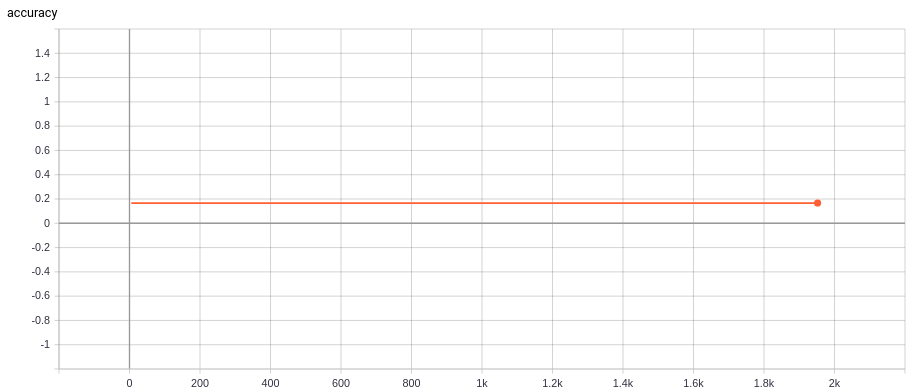
\includegraphics[scale=0.43]{img/player_acc_chap4.png}
	\caption{Akurasi saat \textit{training} pada karakter pemain.}
	\label{fig:nn_player_acc_chap4}
	\vspace{4ex}
	
	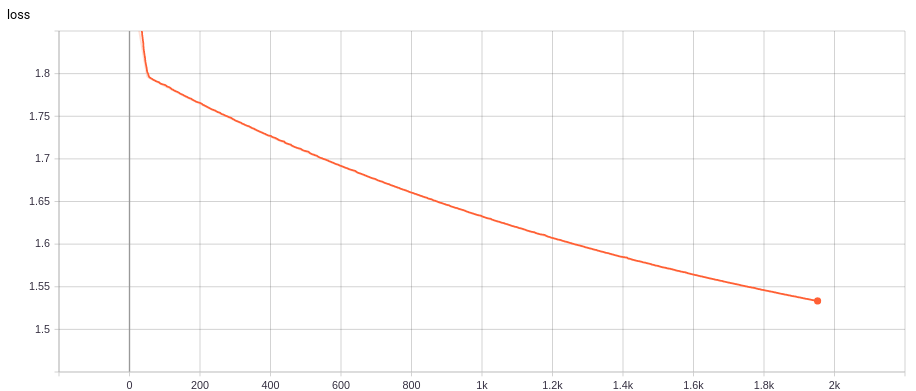
\includegraphics[scale=0.43]{img/player_loss_chap4.png}
	\caption{\textit{Loss} saat \textit{training} pada karakter pemain.}
	\label{fig:nn_player_loss_chap4}
\end{figure}
\clearpage

\begin{figure} [!h] \centering
	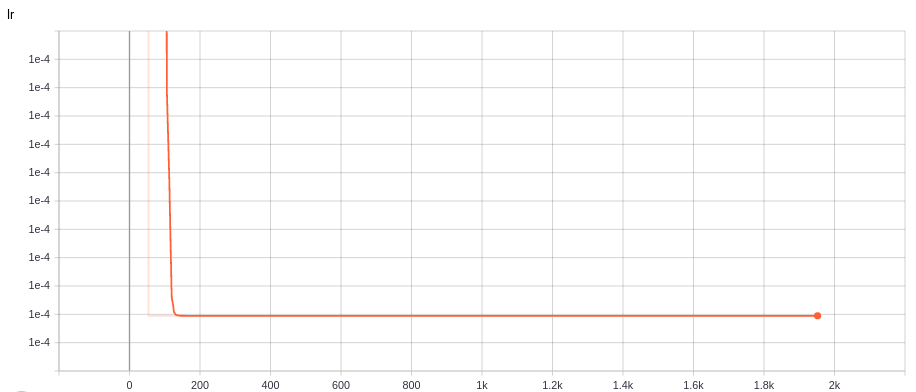
\includegraphics[scale=0.44]{img/player_lr_chap4.png}
	\caption{\textit{Learning rate} saat \textit{training} pada karakter pemain.}
	\label{fig:nn_player_lr_chap4}
	\vspace{4ex}
	
	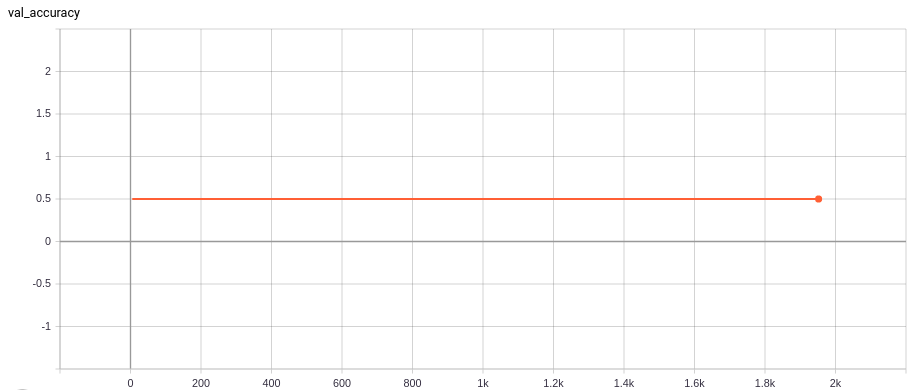
\includegraphics[scale=0.44]{img/player_val_acc_chap4.png}
	\caption{Akurasi pada saat proses evaluasi pada karakter pemain.}
	\label{fig:nn_player_val_acc_chap4}
	\vspace{4ex}
	
	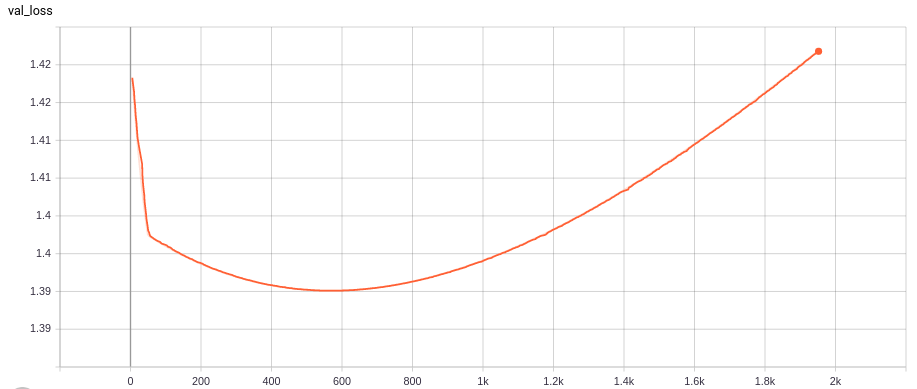
\includegraphics[scale=0.44]{img/player_val_loss_chap4.png}
	\caption{\textit{Loss} saat proses evaluasi pada karakter pemain.}
	\label{fig:nn_player_val_loss_chap4}
\end{figure}
\clearpage

Seperti penjelasan tentang proses \textit{training} pada Sub-bab \ref{sec:sub_sec3_player_char_train}, \textit{training} berlangsung selama 425 \textit{epoch}. Akurasi saat \textit{training} tetap stabil pada 0.1667 dan mengalami \textit{loss} sebesar 1.533, kemudian akurasi saat evaluasi tetap stabil pada 0.5 dan mengalami \textit{loss} saat evaluasisebesar 1.39. Hasil klasifikasi dari data atribut \textit{gameplay} dari karakter pemain yang dijadikan sebagai data \textit{testing} dapat dilihat pada Tabel \ref{tb:player_char_test} yang kemudian digunakan pada proses evaluasi dan \textit{testing} dengan hasil yang ditampilkan pada Tabel \ref{tb:player_valid_result}.
\vspace{-1ex}

\begin{longtable}{|l|l|l|l|l|}
	\caption{Hasil proses \textit{testing} dengan data \textit{testing} pada karakter pemain.}
	\vspace{1ex}
	\label{tb:player_valid_result}\\
	\hline
	\rowcolor[HTML]{C0C0C0} 
	\textbf{Type} & \textbf{Knight} & \textbf{Priest} & \textbf{Assassin} & \textbf{Magician} \\ \hline
	\textbf{Assassin 2} & 0.122532 & 0.190597 & {\color[HTML]{009901} 0.579998} & 0.106873 \\ \hline
	\textbf{Magician 2} & 0.122532 & 0.190597 & {\color[HTML]{FE0000} 0.579998} & 0.106873 \\ \hline
\end{longtable}
\vspace{1ex}

Cara membaca hasil klasifikasi pada Tabel \ref{tb:player_valid_result} sebelumnya sudah dijelaskan pada Sub-bab \ref{sec:sub_sec3_player_arch} dan Sub-bab \ref{sec:sub_sec3_player_char_train}. Hasil ditampilkan pada Tabel \ref{tb:player_valid_result} terdapat satu karakter yang mengalami salah klasifikasi yang kemudian diberi warna merah, dengan beracuan pada Tabel \ref{tb:player_char_test} pada bagian kolom \textit{type}. Maka dari 2 karakter tersebut, terdapat 1 karakter yang mengalami salah klasifikasi atau dianggap tidak sesuai dengan tipenya, bila dinyatakan dalam presentase menjadi 50\% karakter pemain berhasil terklasifikasi.
\vspace{1ex}

\section{Hasil Klasifikasi Karakter Musuh}
\label{sec:sec4_eval_enemy}
\vspace{1ex}

Pada Sub-bab ini akan membahas hasil dari Sub-bab \ref{sec:sec3_enemy_method}, bila dijelaskan melalui diagram blok pada Gambar \ref{fig:enemy_class_proc} maka bagian yang akan dibahas pada Sub-bab ini adalah klasifikasi. Grafik hasil \textit{training} dapat dilihat pada Gambar \ref{fig:nn_enemy_acc_chap4}, \ref{fig:nn_enemy_loss_chap4}, \ref{fig:nn_enemy_lr_chap4}, \ref{fig:nn_enemy_val_acc_chap4}, dan Gambar \ref{fig:nn_enemy_val_loss_chap4}. Masing-masing dari Gambar tersebut secara berurutan diantaranya adalah akurasi saat \textit{training}, \textit{loss} saat \textit{training}, \textit{learning rate} saat \textit{training}, akurasi saat evaluasu dan \textit{loss} saat evaluasi. Pada proses tersebut dijalankan dengan maksimum 20k \textit{epoch}, dengan optimasi sama seperti yang sudah dilakukan dan dijelaskan sebelumnya pada Sub-bab \ref{sec:sub_sec3_dota2_train} dan Sub-bab \ref{sec:sub_sec3_dota2_model}.
\vspace{1ex}

\begin{figure} [!h] \centering
	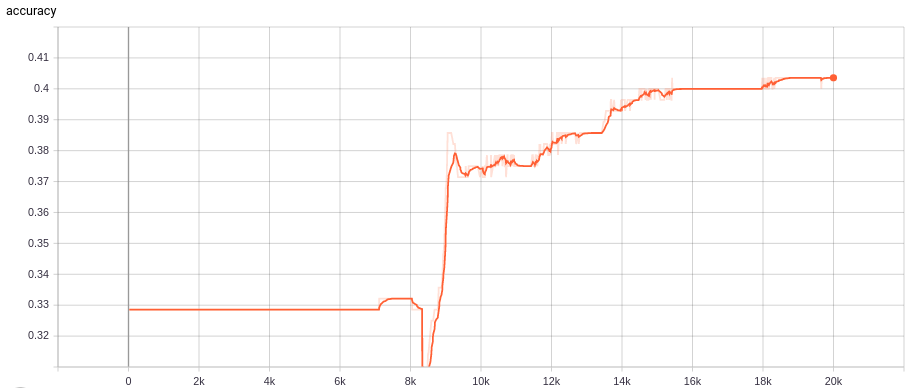
\includegraphics[scale=0.44]{img/enemy_acc_chap4.png}
	\caption{Akurasi saat \textit{training} pada karakter musuh (20k \textit{epoch}).}
	\label{fig:nn_enemy_acc_chap4}
	\vspace{4ex}
	
	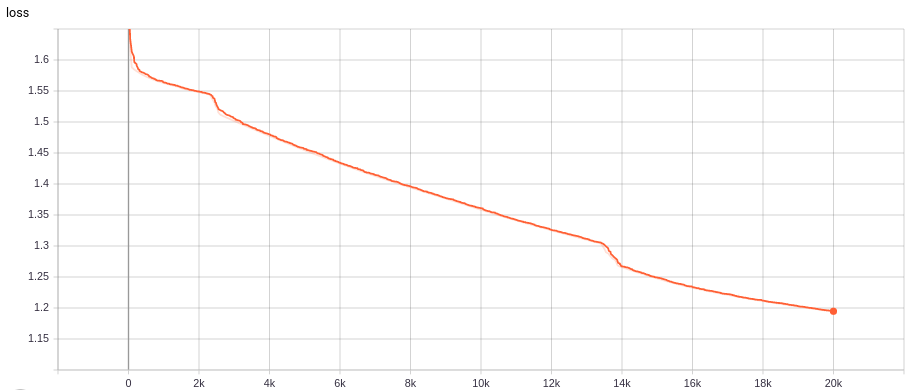
\includegraphics[scale=0.44]{img/enemy_loss_chap4.png}
	\caption{\textit{Loss} saat \textit{training} pada karakter musuh (20k \textit{epoch}).}
	\label{fig:nn_enemy_loss_chap4}
	\vspace{4ex}
	
	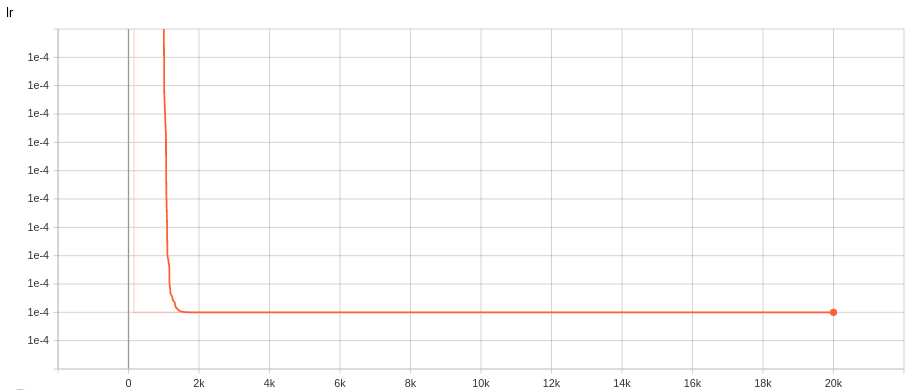
\includegraphics[scale=0.44]{img/enemy_lr_chap4.png}
	\caption{\textit{Learning rate} saat \textit{training} pada karakter musuh (20k \textit{epoch}).}
	\label{fig:nn_enemy_lr_chap4}
\end{figure}
\clearpage

\begin{figure} [!h] \centering
	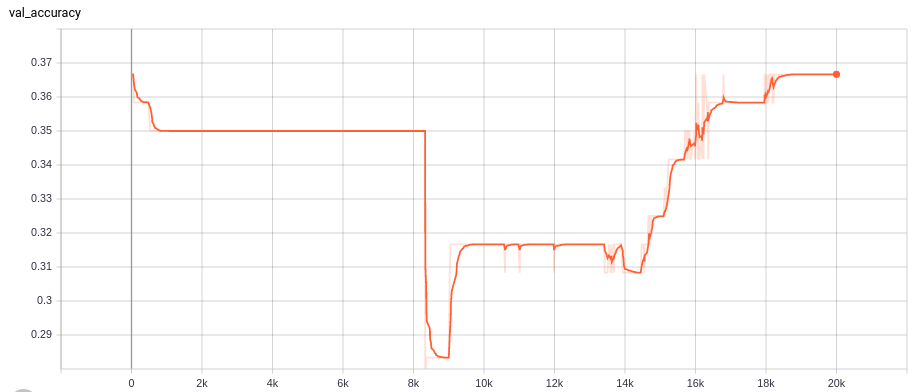
\includegraphics[scale=0.42]{img/enemy_val_acc_chap4.png}
	\caption{Akurasi saat proses evaluasi pada karakter (20k \textit{epoch}).}
	\label{fig:nn_enemy_val_acc_chap4}
	\vspace{4ex}
	
	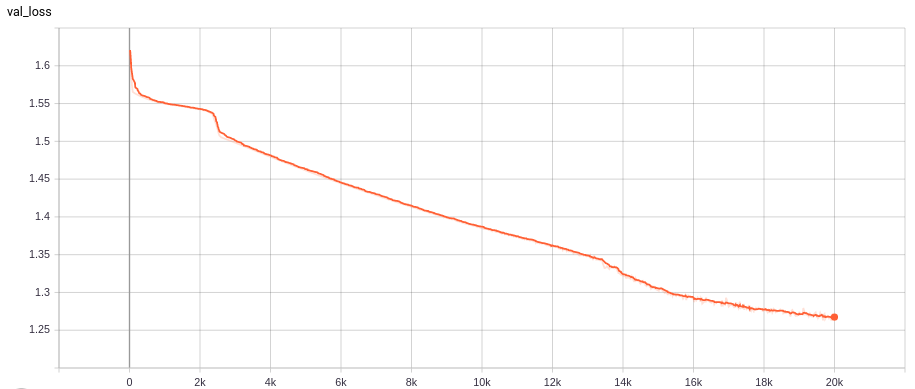
\includegraphics[scale=0.42]{img/enemy_val_loss_chap4.png}
	\caption{\textit{Loss} proses evaluasi pada karakter pemain (20k \textit{epoch}).}
	\label{fig:nn_enemy_val_loss_chap4}
	\vspace{-1ex}
\end{figure}

Seperti penjelasan tentang proses \textit{training} pada Sub-bab \ref{sec:sub_sec3_enemy_char_train}, \textit{training} berlangsung selama 20k \textit{epoch}. Akurasi saat \textit{training} mampu mencapai 0.4 dan mengalami \textit{loss} sebesar 1.194, kemudian akurasi saat \textit{training} mampu mencapai 0.3667 dan mengalami \textit{loss} saat evaluasi sebesar 1.266. Melihat kondisi ini maka dilakukan peningkatan \textit{epoch} menjadi 40k, hal tersebut bertujuan agar tercapainya kondisi optimum. Maksud dari kondisi tersebut adalah dicapainya nilai \textit{loss} terendah saat dilakukannya evaluasi. Grafik hasil \textit{training} dapat dilihat pada Gambar \ref{fig:nn_enemy_acc_40k_chap4}, \ref{fig:nn_enemy_loss_40k_chap4}, \ref{fig:nn_enemy_lr_40k_chap4}, \ref{fig:nn_enemy_val_acc_40k_chap4}, dan Gambar \ref{fig:nn_enemy_val_loss_40k_chap4}. Urutan dari gambar tersebut diantaranya adalah akurasi saat \textit{training}, \textit{loss} saat \textit{training}, \textit{learning rate} saat \textit{training}, akurasi saat evaluasi dan \textit{loss} saat evaluasi dengan 40k \textit{epoch}.

\begin{figure} [!h] \centering
	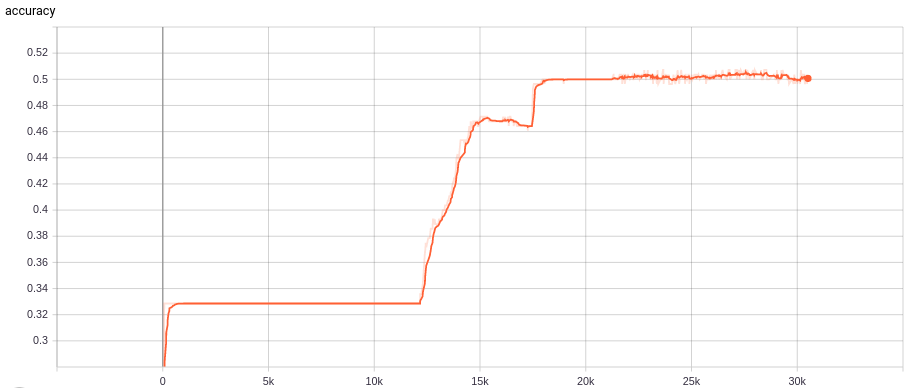
\includegraphics[scale=0.44]{img/enemy_acc_40k_chap4.png}
	\caption{Akurasi saat \textit{training} pada karakter musuh (40k \textit{epoch}).}
	\label{fig:nn_enemy_acc_40k_chap4}
	\vspace{4ex}
	
	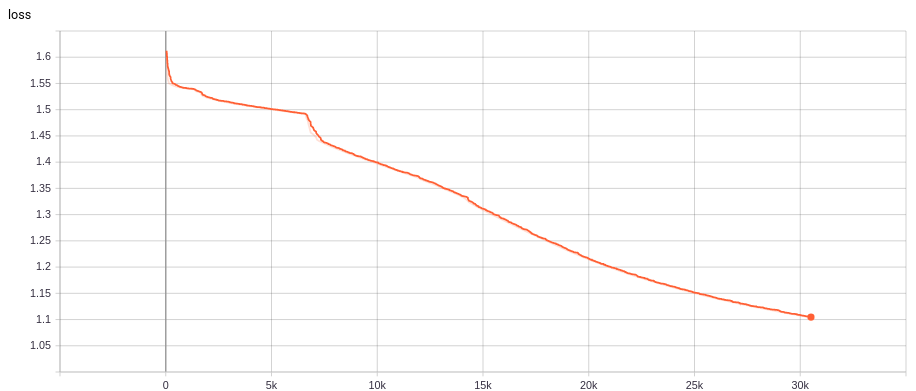
\includegraphics[scale=0.44]{img/enemy_loss_40k_chap4.png}
	\caption{\textit{Loss} saat \textit{training} pada karakter musuh (40k \textit{epoch}).}
	\label{fig:nn_enemy_loss_40k_chap4}
	\vspace{4ex}
	
	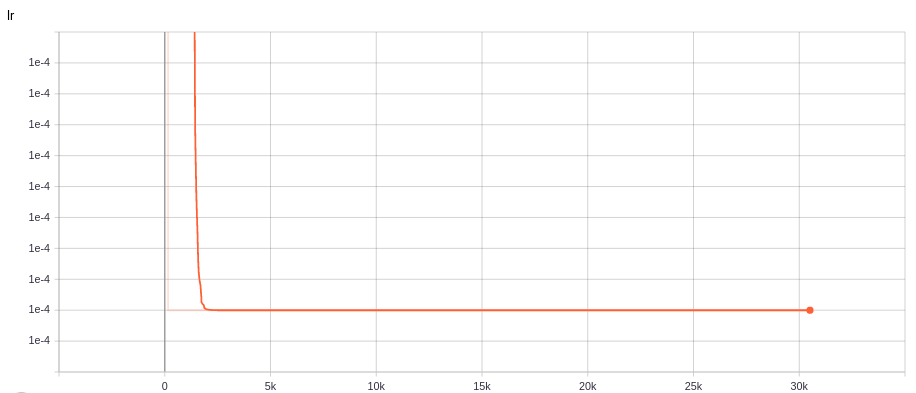
\includegraphics[scale=0.44]{img/enemy_lr_40k_chap4.png}
	\caption{\textit{Learning rate} saat \textit{training} pada karakter musuh (40k \textit{epoch}).}
	\label{fig:nn_enemy_lr_40k_chap4}
\end{figure}
\clearpage

\begin{figure} [!h] \centering
	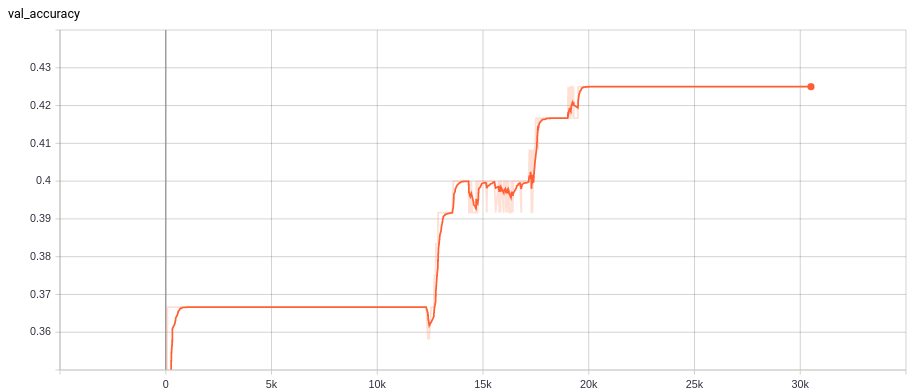
\includegraphics[scale=0.42]{img/enemy_val_acc_40k_chap4.png}
	\caption{Akurasi saat evaluasi pada karakter musuh (40k \textit{epoch}).}
	\label{fig:nn_enemy_val_acc_40k_chap4}
	\vspace{4ex}
	
	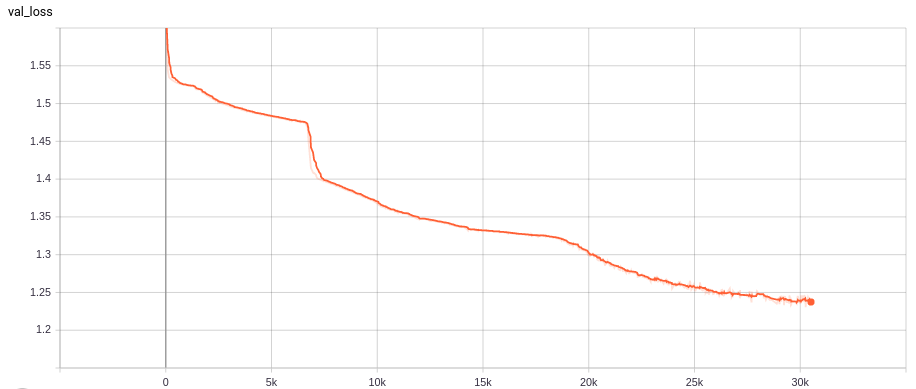
\includegraphics[scale=0.42]{img/enemy_val_loss_40k_chap4.png}
	\caption{\textit{Loss} saat evaluasi pada karakter musuh (40k \textit{epoch}).}
	\label{fig:nn_enemy_val_loss_40k_chap4}
\end{figure}

Seperti penjelasan tentang proses \textit{training} pada Sub-bab \ref{sec:sub_sec3_enemy_char_train}, \textit{training} berlangsung selama 30.510 \textit{epoch} setelah dilakukan penambahan 20k \textit{epoch}, yang semula hanya 20k \textit{epoch} menjadi 40k \textit{epoch}. Hal tersebut diasumsikan bahwa kondisi optimum dapat dicapai dengan \textit{epoch} kurang dari 40k dan lebih dari 20k. Akurasi saat \textit{training} mampu mencapai 0.5 dan mengalami \textit{loss} sebesar 1.110, kemudian akurasi saat evaluasi mampu mencapai 0.425 dan mengalami \textit{loss} saat evaluasi sebesar 1.245. Hasil klasifikasi dari data atribut \textit{gameplay} karakter musuh yang dijadikan sebagai data evaluasi dapat dilihat pada Tabel \ref{tb:enemy_all_stats_1} sampai dengan Tabel \ref{tb:enemy_all_stats_15} untuk musuh dengan urutan ke 281 sampai 400, kemudian data tersebut digunakan pada proses evaluasi dan \textit{testing} dengan hasil yang dapat dilihat pada Tabel \ref{tb:enemy_valid_result}.
\vspace{-2ex}

\begin{longtable}{|l|l|l|l|l|l|l|}
	\caption{Hasil proses \textit{testing} dengan data \textit{testing} pada karakter musuh.}
	\vspace{1ex}
	\label{tb:enemy_valid_result}\\
	\hline
	\rowcolor[HTML]{C0C0C0} 
	\textbf{Name} & \textbf{Type} & \textbf{Type 0} & \textbf{Type 1} & \textbf{Type 2} & \textbf{Type 3} & \textbf{Type 4} \\ \hline
	Enemy 281 & 2 & 0.378368 & {\color[HTML]{FE0000} 0.168215} & 0.316104 & 0.058081 & 0.079233 \\ \hline
	Enemy 282 & 0 & {\color[HTML]{FE0000} 0.527585} & 0.010544 & 0.046145 & 0.122267 & 0.293459 \\ \hline
	Enemy 283 & 2 & 0.371143 & 0.13154 & {\color[HTML]{FE0000} 0.276541} & 0.092394 & 0.128382 \\ \hline
	Enemy 284 & 1 & 0.374915 & {\color[HTML]{FE0000} 0.187169} & 0.332138 & 0.044986 & 0.060792 \\ \hline
	Enemy 285 & 4 & 0.524063 & 0.010682 & 0.046597 & 0.123526 & {\color[HTML]{FE0000} 0.295132} \\ \hline
	Enemy 286 & 0 & {\color[HTML]{009901} 0.374915} & 0.187169 & 0.332138 & 0.044986 & 0.060792 \\ \hline
	Enemy 287 & 1 & 0.374915 & {\color[HTML]{FE0000} 0.187169} & 0.332138 & 0.044986 & 0.060792 \\ \hline
	Enemy 288 & 0 & {\color[HTML]{FE0000} 0.374915} & 0.187169 & 0.332138 & 0.044986 & 0.060792 \\ \hline
	Enemy 289 & 2 & 0.377502 & 0.175532 & {\color[HTML]{FE0000} 0.322636} & 0.0527 & 0.07163 \\ \hline
	Enemy 290 & 0 & {\color[HTML]{009901} 0.37244} & 0.191845 & 0.329262 & 0.045204 & 0.06125 \\ \hline
	Enemy 291 & 1 & 0.44503 & {\color[HTML]{FE0000} 0.158904} & 0.29768 & 0.039981 & 0.058406 \\ \hline
	Enemy 292 & 0 & {\color[HTML]{009901} 0.527579} & 0.010545 & 0.046146 & 0.122269 & 0.293462 \\ \hline
	Enemy 293 & 0 & {\color[HTML]{009901} 0.374915} & 0.187169 & 0.332138 & 0.044986 & 0.060792 \\ \hline
	Enemy 294 & 2 & 0.375155 & 0.186315 & {\color[HTML]{FE0000} 0.331476} & 0.045518 & 0.061537 \\ \hline
	Enemy 295 & 0 & {\color[HTML]{009901} 0.374915} & 0.187169 & 0.332138 & 0.044986 & 0.060792 \\ \hline
	Enemy 296 & 0 & {\color[HTML]{009901} 0.39901} & 0.177068 & 0.320346 & 0.043361 & 0.060215 \\ \hline
	Enemy 297 & 0 & {\color[HTML]{009901} 0.374915} & 0.187169 & 0.332138 & 0.044986 & 0.060792 \\ \hline
	Enemy 298 & 1 & 0.779063 & {\color[HTML]{FE0000} 0.049134} & 0.121837 & 0.015684 & 0.034281 \\ \hline
	Enemy 299 & 2 & 0.374915 & 0.187168 & {\color[HTML]{FE0000} 0.332138} & 0.044986 & 0.060793 \\ \hline
	Enemy 300 & 3 & 0.19636 & 0.031101 & 0.097399 & {\color[HTML]{FE0000} 0.271855} & 0.403286 \\ \hline
	Enemy 301 & 4 & 0.198122 & 0.030917 & 0.097056 & 0.270797 & {\color[HTML]{009901} 0.403107} \\ \hline
	Enemy 302 & 0 & {\color[HTML]{009901} 0.360234} & 0.114637 & 0.254198 & 0.112808 & 0.158123 \\ \hline
	Enemy 303 & 2 & 0.374915 & 0.187169 & {\color[HTML]{FE0000} 0.332138} & 0.044986 & 0.060792 \\ \hline
	Enemy 304 & 0 & {\color[HTML]{009901} 0.374915} & 0.187169 & 0.332138 & 0.044986 & 0.060792 \\ \hline
	Enemy 305 & 1 & 0.374915 & {\color[HTML]{FE0000} 0.187169} & 0.332138 & 0.044986 & 0.060792 \\ \hline
	Enemy 306 & 0 & {\color[HTML]{009901} 0.431493} & 0.01471 & 0.059049 & 0.158573 & 0.336175 \\ \hline
	Enemy 307 & 2 & 0.355833 & 0.109533 & {\color[HTML]{FE0000} 0.246909} & 0.119611 & 0.168114 \\ \hline
	Enemy 308 & 1 & 0.247685 & {\color[HTML]{009901} 0.432672} & 0.201979 & 0.047006 & 0.070658 \\ \hline
	Enemy 309 & 0 & {\color[HTML]{009901} 0.375144} & 0.187072 & 0.332027 & 0.04497 & 0.060786 \\ \hline
	Enemy 310 & 0 & {\color[HTML]{009901} 0.489814} & 0.012073 & 0.051075 & 0.136044 & 0.310994 \\ \hline
	Enemy 311 & 1 & 0.374915 & {\color[HTML]{FE0000} 0.187169} & 0.332138 & 0.044986 & 0.060792 \\ \hline
	Enemy 312 & 0 & {\color[HTML]{FE0000} 0.196372} & 0.0311 & 0.097396 & 0.271848 & 0.403284 \\ \hline
	Enemy 313 & 2 & 0.374975 & 0.186958 & {\color[HTML]{FE0000} 0.331975} & 0.045117 & 0.060975 \\ \hline
	Enemy 314 & 4 & 0.196605 & 0.031075 & 0.097351 & 0.271708 & {\color[HTML]{009901} 0.403261} \\ \hline
	Enemy 315 & 0 & {\color[HTML]{009901} 0.759012} & 0.053907 & 0.13179 & 0.017714 & 0.037577 \\ \hline
	Enemy 316 & 2 & 0.300307 & 0.069685 & {\color[HTML]{FE0000} 0.180658} & 0.184301 & 0.26505 \\ \hline
	Enemy 317 & 1 & 0.374915 & {\color[HTML]{FE0000} 0.187169} & 0.332138 & 0.044986 & 0.060792 \\ \hline
	Enemy 318 & 0 & {\color[HTML]{009901} 0.37831} & 0.168413 & 0.316292 & 0.057946 & 0.079039 \\ \hline
	Enemy 319 & 2 & 0.374928 & 0.187163 & {\color[HTML]{FE0000} 0.332131} & 0.044985 & 0.060792 \\ \hline
	Enemy 320 & 3 & 0.19636 & 0.031101 & 0.097399 & {\color[HTML]{FE0000} 0.271855} & 0.403286 \\ \hline
	Enemy 321 & 2 & 0.374915 & 0.187168 & {\color[HTML]{FE0000} 0.332138} & 0.044986 & 0.060793 \\ \hline
	Enemy 322 & 0 & {\color[HTML]{009901} 0.527585} & 0.010544 & 0.046145 & 0.122267 & 0.293459 \\ \hline
	Enemy 323 & 2 & 0.378495 & 0.162733 & {\color[HTML]{FE0000} 0.310932} & 0.062436 & 0.085403 \\ \hline
	Enemy 324 & 4 & 0.197093 & 0.031301 & 0.097895 & 0.271315 & {\color[HTML]{009901} 0.402396} \\ \hline
	Enemy 325 & 4 & 0.525411 & 0.010629 & 0.046424 & 0.123043 & {\color[HTML]{FE0000} 0.294493} \\ \hline
	Enemy 326 & 3 & 0.196361 & 0.031101 & 0.097399 & {\color[HTML]{FE0000} 0.271854} & 0.403285 \\ \hline
	Enemy 327 & 0 & {\color[HTML]{009901} 0.527585} & 0.010544 & 0.046145 & 0.122267 & 0.293459 \\ \hline
	Enemy 328 & 2 & 0.37741 & 0.176108 & {\color[HTML]{FE0000} 0.323131} & 0.052294 & 0.071056 \\ \hline
	Enemy 329 & 4 & 0.203998 & 0.033222 & 0.102619 & 0.266182 & {\color[HTML]{009901} 0.393979} \\ \hline
	Enemy 330 & 2 & 0.377303 & 0.176747 & {\color[HTML]{FE0000} 0.323677} & 0.051846 & 0.070426 \\ \hline
	Enemy 331 & 0 & {\color[HTML]{009901} 0.374915} & 0.187168 & 0.332138 & 0.044986 & 0.060793 \\ \hline
	Enemy 332 & 1 & 0.374915 & 0.187169 & 0.332138 & 0.044986 & 0.060792 \\ \hline
	Enemy 333 & 0 & {\color[HTML]{009901} 0.377455} & 0.175831 & 0.322893 & 0.052489 & 0.071332 \\ \hline
	Enemy 334 & 1 & 0.374915 & {\color[HTML]{FE0000} 0.187169} & 0.332138 & 0.044986 & 0.060792 \\ \hline
	Enemy 335 & 0 & {\color[HTML]{FE0000} 0.19636} & 0.031101 & 0.097399 & 0.271855 & 0.403286 \\ \hline
	Enemy 336 & 4 & 0.196498 & 0.031087 & 0.097372 & 0.271772 & {\color[HTML]{009901} 0.403272} \\ \hline
	Enemy 337 & 0 & {\color[HTML]{009901} 0.374915} & 0.187169 & 0.332138 & 0.044986 & 0.060792 \\ \hline
	Enemy 338 & 4 & 0.288799 & 0.023111 & 0.080821 & 0.221746 & {\color[HTML]{009901} 0.385523} \\ \hline
	Enemy 339 & 0 & {\color[HTML]{009901} 0.374915} & 0.187169 & 0.332138 & 0.044986 & 0.060792 \\ \hline
	Enemy 340 & 0 & {\color[HTML]{009901} 0.527585} & 0.010544 & 0.046145 & 0.122267 & 0.293459 \\ \hline
	Enemy 341 & 0 & {\color[HTML]{009901} 0.374915} & 0.187169 & 0.332138 & 0.044986 & 0.060792 \\ \hline
	Enemy 342 & 2 & 0.339119 & 0.094142 & {\color[HTML]{FE0000} 0.223345} & 0.142054 & 0.20134 \\ \hline
	Enemy 343 & 0 & {\color[HTML]{009901} 0.374915} & 0.187169 & 0.332138 & 0.044986 & 0.060792 \\ \hline
	Enemy 344 & 3 & 0.19636 & 0.031101 & 0.097399 & {\color[HTML]{FE0000} 0.271855} & 0.403286 \\ \hline
	Enemy 345 & 2 & 0.344267 & 0.098384 & {\color[HTML]{FE0000} 0.230083} & 0.135569 & 0.191696 \\ \hline
	Enemy 346 & 2 & 0.374915 & 0.187169 & {\color[HTML]{FE0000} 0.332138} & 0.044986 & 0.060792 \\ \hline
	Enemy 347 & 3 & 0.19636 & 0.031101 & 0.097399 & {\color[HTML]{FE0000} 0.271855} & 0.403286 \\ \hline
	Enemy 348 & 0 & {\color[HTML]{009901} 0.389206} & 0.175524 & 0.320846 & 0.048171 & 0.066253 \\ \hline
	Enemy 349 & 4 & 0.196971 & 0.031037 & 0.09728 & 0.271487 & {\color[HTML]{009901} 0.403225} \\ \hline
	Enemy 350 & 2 & 0.376953 & 0.178691 & {\color[HTML]{FE0000} 0.325319} & 0.050502 & 0.068535 \\ \hline
	Enemy 351 & 4 & 0.527585 & 0.010544 & 0.046145 & 0.122267 & {\color[HTML]{FE0000} 0.293459} \\ \hline
	Enemy 352 & 2 & 0.343683 & 0.097884 & {\color[HTML]{FE0000} 0.229299} & 0.136321 & 0.192813 \\ \hline
	Enemy 353 & 1 & {\color[HTML]{FE0000} 0.374915} & 0.187169 & 0.332138 & 0.044986 & 0.060792 \\ \hline
	Enemy 354 & 0 & {\color[HTML]{009901} 0.375058} & 0.186662 & 0.331746 & 0.045301 & 0.061233 \\ \hline
	Enemy 355 & 0 & {\color[HTML]{009901} 0.527585} & 0.010544 & 0.046145 & 0.122267 & 0.293459 \\ \hline
	Enemy 356 & 2 & 0.374915 & 0.187169 & {\color[HTML]{FE0000} 0.332138} & 0.044986 & 0.060792 \\ \hline
	Enemy 357 & 3 & 0.524283 & 0.010673 & 0.046569 & {\color[HTML]{FE0000} 0.123447} & 0.295028 \\ \hline
	Enemy 358 & 0 & {\color[HTML]{FE0000} 0.19636} & 0.031101 & 0.097399 & 0.271855 & 0.403286 \\ \hline
	Enemy 359 & 4 & 0.19636 & 0.031101 & 0.097399 & 0.271855 & {\color[HTML]{009901} 0.403286} \\ \hline
	Enemy 360 & 0 & {\color[HTML]{FE0000} 0.22214} & 0.038611 & 0.115484 & 0.252301 & 0.371463 \\ \hline
	Enemy 361 & 2 & 0.376041 & 0.182882 & {\color[HTML]{FE0000} 0.328761} & 0.047708 & 0.064608 \\ \hline
	Enemy 362 & 2 & 0.374919 & 0.187166 & {\color[HTML]{FE0000} 0.332135} & 0.044987 & 0.060793 \\ \hline
	Enemy 363 & 1 & 0.247685 & {\color[HTML]{009901} 0.432672} & 0.201979 & 0.047006 & 0.070658 \\ \hline
	Enemy 364 & 0 & {\color[HTML]{FE0000} 0.19636} & 0.031101 & 0.097399 & 0.271855 & 0.403286 \\ \hline
	Enemy 365 & 2 & 0.290789 & 0.064962 & {\color[HTML]{FE0000} 0.171607} & 0.193501 & 0.279142 \\ \hline
	Enemy 366 & 4 & 0.377982 & 0.171986 & 0.319527 & 0.055262 & {\color[HTML]{FE0000} 0.075243} \\ \hline
	Enemy 367 & 0 & {\color[HTML]{009901} 0.374912} & 0.187175 & 0.332134 & 0.044987 & 0.060793 \\ \hline
	Enemy 368 & 3 & 0.523421 & 0.010707 & 0.04668 & {\color[HTML]{FE0000} 0.123756} & 0.295437 \\ \hline
	Enemy 369 & 4 & 0.526284 & 0.010595 & 0.046312 & 0.122731 & {\color[HTML]{FE0000} 0.294078} \\ \hline
	Enemy 370 & 4 & 0.527563 & 0.010545 & 0.046148 & 0.122274 & {\color[HTML]{FE0000} 0.293469} \\ \hline
	Enemy 371 & 0 & {\color[HTML]{009901} 0.527623} & 0.010546 & 0.04615 & 0.122254 & 0.293427 \\ \hline
	Enemy 372 & 0 & {\color[HTML]{009901} 0.380983} & 0.15926 & 0.307262 & 0.064246 & 0.08825 \\ \hline
	Enemy 373 & 0 & {\color[HTML]{009901} 0.375367} & 0.185541 & 0.330872 & 0.046004 & 0.062218 \\ \hline
	Enemy 374 & 1 & 0.374915 & {\color[HTML]{FE0000} 0.187169} & 0.332138 & 0.044986 & 0.060792 \\ \hline
	Enemy 375 & 1 & 0.374915 & {\color[HTML]{FE0000} 0.187169} & 0.332138 & 0.044986 & 0.060792 \\ \hline
	Enemy 376 & 0 & {\color[HTML]{009901} 0.4574} & 0.013494 & 0.05545 & 0.148368 & 0.325289 \\ \hline
	Enemy 377 & 0 & {\color[HTML]{FE0000} 0.247685} & 0.432672 & 0.201979 & 0.047006 & 0.070658 \\ \hline
	Enemy 378 & 4 & 0.201898 & 0.032631 & 0.101173 & 0.267752 & {\color[HTML]{009901} 0.396547} \\ \hline
	Enemy 379 & 4 & 0.485689 & 0.012248 & 0.051624 & 0.137586 & {\color[HTML]{FE0000} 0.312853} \\ \hline
	Enemy 380 & 2 & 0.378341 & 0.167954 & {\color[HTML]{FE0000} 0.315869} & 0.058299 & 0.079537 \\ \hline
	Enemy 381 & 0 & {\color[HTML]{FE0000} 0.247685} & 0.432672 & 0.201979 & 0.047006 & 0.070658 \\ \hline
	Enemy 382 & 2 & 0.373738 & 0.137479 & {\color[HTML]{FE0000} 0.283757} & 0.085953 & 0.119072 \\ \hline
	Enemy 383 & 3 & 0.773596 & 0.046859 & 0.119864 & {\color[HTML]{FE0000} 0.018757} & 0.040924 \\ \hline
	Enemy 384 & 0 & {\color[HTML]{009901} 0.46142} & 0.013312 & 0.0549 & 0.146813 & 0.323555 \\ \hline
	Enemy 385 & 3 & 0.196482 & 0.031088 & 0.097375 & {\color[HTML]{FE0000} 0.271781} & 0.403274 \\ \hline
	Enemy 386 & 3 & 0.19636 & 0.031101 & 0.097399 & {\color[HTML]{FE0000} 0.271855} & 0.403286 \\ \hline
	Enemy 387 & 1 & 0.374915 & {\color[HTML]{FE0000} 0.187169} & 0.332138 & 0.044986 & 0.060792 \\ \hline
	Enemy 388 & 3 & 0.196366 & 0.0311 & 0.097397 & {\color[HTML]{FE0000} 0.271851} & 0.403285 \\ \hline
	Enemy 389 & 0 & {\color[HTML]{009901} 0.375897} & 0.183475 & 0.329236 & 0.047324 & 0.064068 \\ \hline
	Enemy 390 & 1 & 0.247687 & {\color[HTML]{009901} 0.432668} & 0.201981 & 0.047006 & 0.070658 \\ \hline
	Enemy 391 & 4 & 0.196473 & 0.031132 & 0.097475 & 0.271772 & {\color[HTML]{009901} 0.403148} \\ \hline
	Enemy 392 & 1 & 0.374915 & {\color[HTML]{FE0000} 0.187169} & 0.332138 & 0.044986 & 0.060792 \\ \hline
	Enemy 393 & 4 & 0.19636 & 0.031101 & 0.097399 & 0.271855 & {\color[HTML]{009901} 0.403286} \\ \hline
	Enemy 394 & 4 & 0.19636 & 0.031101 & 0.097399 & 0.271855 & {\color[HTML]{009901} 0.403286} \\ \hline
	Enemy 395 & 0 & {\color[HTML]{009901} 0.374914} & 0.18717 & 0.332137 & 0.044986 & 0.060793 \\ \hline
	Enemy 396 & 0 & {\color[HTML]{FE0000} 0.242251} & 0.026766 & 0.088846 & 0.245748 & 0.39639 \\ \hline
	Enemy 397 & 1 & 0.374915 & {\color[HTML]{FE0000} 0.187169} & 0.332138 & 0.044986 & 0.060792 \\ \hline
	Enemy 398 & 1 & 0.374915 & {\color[HTML]{FE0000} 0.187169} & 0.332138 & 0.044986 & 0.060792 \\ \hline
	Enemy 399 & 3 & 0.19636 & 0.031101 & 0.097399 & {\color[HTML]{FE0000} 0.271855} & 0.403286 \\ \hline
	Enemy 400 & 3 & 0.19636 & 0.031101 & 0.097399 & {\color[HTML]{FE0000} 0.271855} & 0.403286 \\ \hline
\end{longtable}
\vspace{1ex}

Cara membaca hasil klasifikasi pada Tabel \ref{tb:player_valid_result} sebelumnya sudah dijelaskan pada Sub-bab \ref{sec:sub_sec3_enemy_arch} dan Sub-bab \ref{sec:sub_sec3_enemy_char_train}. Hasil ditampilkan pada Tabel \ref{tb:enemy_valid_result} terdapat 51 karakter yang terklasifikasi dengan benar atau sesuai dengan tipe saat karakter musuh dibuat. Kemudian pada karakter tersebut setiap angka tingkat keyakinan ditandai dengan warna hijau, dengan beracuan pada pada Tabel \ref{tb:enemy_all_stats_1} sampai dengan Tabel \ref{tb:enemy_all_stats_15} untuk musuh dengan urutan ke 281 sampai 400 pada bagian kolom \textit{type}. Maka dari 120 karakter tersebut, terdapat 51 karakter yang berhasil terklasifikasi, bila dinyatakan dalam presentase maka menjadi 42.5\% karakter pemain berhasil terklasifikasi.